\documentclass[]{beamer}
\usepackage{etoolbox} % true false
\providetoggle{thesis}\settoggle{thesis}{true}
\providetoggle{plots}\settoggle{plots}{true}
\providetoggle{beamer}\settoggle{beamer}{true}
\providetoggle{final}\settoggle{final}{true} % use smaller plots etc
\usepackage{lmodern} % Use an extension of the original Computer Modern font to minimize the use of bitmapped letters.
\usepackage{listings}
\renewcommand{\ttdefault}{pcr} % different monospace font with bfseries
\usepackage[T1]{fontenc}    % Determines font encoding of the output. Font packages have to be included before this line.
\usepackage[utf8]{inputenc} % Determines encoding of the input. All input files have to use UTF8 encoding.
\usepackage{graphicx}
\usepackage{xspace}

% Extended LaTeX functionality is enables by including packages with \usepackage{...}.
\usepackage{amsmath}    % Extended typesetting of mathematical expression.
\usepackage{amssymb}    % Provides a multitude of mathematical symbols.
\usepackage{mathtools}  % Further extensions of mathematical typesetting.
\usepackage{microtype}  % Small-scale typographic enhancements.
\usepackage{multirow}   % Allows table elements to span several rows.
\usepackage{booktabs}   % Improves the type settings of tables.
\usepackage{subcaption} % Allows the use of subfigures and enables their referencing.
%\usepackage[ruled,linesnumbered,algochapter]{algorithm2e} % Enables the writing of pseudo code.
%\usepackage[usenames,dvipsnames,table]{xcolor} % Allows the definition and use of colors. This package has to be included before tikz.
\usepackage{todonotes} % Provides tooltip-like todo notes.
\usepackage{hyperref}  % Enables cross linking in the electronic document version. This package has to be included second to last.
\usepackage[acronym,toc]{glossaries} % Enables the generation of glossaries and lists fo acronyms. This package has to be included last.
\usepackage{marvosym}
\usepackage{nicefrac}
\usepackage{bm}
\usepackage[english]{babel}
\usepackage[]{cleveref}
%% Text highlighting
\usepackage{soul}
\usepackage{soulutf8}
\usepackage{blkarray}
\usepackage{floatpag}

\usepackage{appendixnumberbeamer}
\usepackage{pgfplotstable}
\soulregister\cite7
\soulregister\ref7
\soulregister\cref7
\soulregister\pageref7
\soulregister\citeyear7

\usepackage{tikz}
\usepackage{pgfplots}
\usepackage{float}
%\usepackage[ruled,vlined]{algorithm2e}
%\usepackage{nicefrac}


% Theorems etc

\iftoggle{beamer}{}{
    \usepackage{ntheorem}
    \newtheorem{definition}{Definition}[chapter]
    \newtheorem{remark}{Remark}[chapter]
}
 
 
 
 \def\nBanks{796\space}
 \def\nCompaniesGephi{5\thinspace000\xspace}
 \def\NWSize{\iftoggle{final}{5000}{500}c}
%  \def\NWSize{500c}

 %
\usetikzlibrary{shapes,backgrounds,calc}
\usetikzlibrary{arrows.meta}
\usetikzlibrary{positioning,graphs}

\definecolor{uvred}{RGB}{255,31,0}
\definecolor{uvblue}{RGB}{0,105,170}

\definecolor{Red}{rgb}{0.89, 0.0, 0.13}
\definecolor{Green}{rgb}{0.01, 0.75, 0.24}
\definecolor{gv}{rgb}{0.61, 0.85, 0.24}
\definecolor{bv}{rgb}{0.26, 0.57, 0.66}
\colorlet{uvblue}{uvblue}
\colorlet{uvbluedark}{black!40!uvblue}
\colorlet{uvbluelight}{white!40!uvblue}


%\usetikzlibrary{pgfplots.clickable}\pgfplotsset{/pgfplots/annot/printable=false}
%\pgfplotsset{compat=1.15}
\pgfplotsset{
%%%%
clickable coords/.style={}, %% comment this line out if coords should be clickable
%%%%
plotl/.style={uvbluelight,no marks,ultra thick,samples=500},
plott/.style={uvblue,no marks,ultra thick,samples=500},
plotd/.style={uvbluedark,no marks,ultra thick,samples=500},
%%
plotA/.style={uvblue!40!white,ultra thick,mark=otimes*},
plotB/.style={uvblue!70!white,ultra thick,mark=triangle*},
plotC/.style={uvblue!90!white,ultra thick,mark=pentagon*},
plotD/.style={uvblue!70!black,ultra thick,mark=diamond*},
plotE/.style={uvblue!50!black,ultra thick,mark=square*},
plotF/.style={uvblue!20!black,ultra thick,mark=otimes},
%plotG/.style={uvblue!20!black,ultra thick,mark=otimes},
%
LplotA/.style={white!10!uvbluelight,ultra thick,},
LplotB/.style={uvbluelight,ultra thick,},
LplotC/.style={uvblue,ultra thick},
LplotD/.style={uvbluedark,ultra thick},
LplotE/.style={black!40!uvbluedark,ultra thick},
LplotF/.style={black!60!uvbluedark,ultra thick},
%
asdfas/.style={}
}

\pgfplotsset{
    discard if not/.style 2 args={
        x filter/.code={
            \edef\tempa{\thisrow{#1}}
            \edef\tempb{#2}
            \ifx\tempa\tempb
            \else
                \def\pgfmathresult{inf}
            \fi
        }
    }
}

\pgfplotstableset{
    discard if not/.style 2 args={
        row predicate/.code={
            \def\pgfplotstable@loc@TMPd{\pgfplotstablegetelem{##1}{#1}\of}
            \expandafter\pgfplotstable@loc@TMPd\pgfplotstablename
            \edef\tempa{\pgfplotsretval}
            \edef\tempb{#2}
            \ifx\tempa\tempb
            \else
                \pgfplotstableuserowfalse
            \fi
        }
    }
}


\pgfplotsset{
    /pgfplots/flexible xticklabels from table/.code n args={3}{%
        \pgfplotstableread[#3]{#1}\coordinate@table
        \pgfplotstablegetcolumn{#2}\of{\coordinate@table}\to\pgfplots@xticklabels
        \let\pgfplots@xticklabel=\pgfplots@user@ticklabel@list@x
    }
}

%% Text shading macros
%\newcommand{\ugly}[1]{\colorbox{blue!30}{#1}\xspace}
\colorlet{hlblue}{uvred!30}
\sethlcolor{hlblue}

% Figure with source Attribution
\newcommand\sourcedFigure[2]{
\begin{tikzpicture}
    \node[] (fig) {#1};
    \node [anchor=south east,color=darkgray,inner sep=0,xshift=-15pt,yshift=0pt]at (fig.north east) {\footnotesize Source: #2};
\end{tikzpicture}}

%: Math macros
\newcommand{\norm}[1]{\left\lvert#1\right\rvert}

% Border around tikzpictures 
\usetikzlibrary{backgrounds}

%: Use colormap for custom charts:
\usepgfplotslibrary{colormaps}
\pgfplotsset{colormap name=viridis}%
\tikzset{
    ellEV/.style={
        % pgfplots/colormap name=viridis,
        color of colormap={200 + #1*1600}, % offset * 2 + scale <= 2000
        draw=.!80!black,
        fill=.!70!white,
        text = black},
    degCen/.style={
        color of colormap={200 + #1 * 800/7}, % offset +  + scale <= 1000
        draw=.!80!black,
        fill=.!70!white,
        text = black
    },
    degCen2/.style={
        color of colormap={300 + #1 * 700/5}, % offset + scale <= 1000
        draw=.!80!black,
        fill=.!70!white,
        text = black
    },
    drMap/.style={
        color of colormap={250 + #1 * 750}, % offset + scale <= 1000
        draw=.!80!black,
        fill=.!70!white,
        text = black
    },
    bankCount/.style={ % between 0 and 6
    ,    color of colormap={#1 * 1000/6} % offset + scale <= 1000
    ,    draw=.!60!black
    ,    fill=.!100!white
    ,    text = black
	},
    onaceColor/.style={ % between 0 and 10
    ,    color of colormap={#1 * 111} % offset + scale <= 1000
    ,    draw=.!60!black
    ,    fill=.!100!white
    ,    text = black
    },
    bankColor/.style={
    ,    color of colormap={850}
    ,    draw=.!70!black
    ,    fill=.!100!white
    ,    text = black
    },
    companyColor/.style={
    ,   color of colormap={400}
    ,   draw=.!70!black
    ,   fill=.!100!white
    ,   text = black
    },
    bankColorLine/.style={
    ,    color of colormap={850}
    ,    draw=.!100!white
    ,    fill=.!100!white
    ,    text = black
    },
    companyColorLine/.style={
    ,   color of colormap={400}
    ,   draw=.!100!white
    ,   fill=.!100!white
    ,   text = black
	},
    depositColor/.style={
    ,   color of colormap={1000}
    ,   draw=.!70!black
    ,   fill=.!100!white
    ,   text = black
	},
	adjMatrix/.style={
    ,   color of colormap={#1 * 825/5 + 125}
    ,   draw=.!100!black
    ,   fill= none
%    ,   text=.!100!black
	},
	diffGlg/.style={ % between 0 and 10
    ,    color of colormap={#1 * 111} % offset + scale <= 1000
%,    draw=.!60!black
%,    fill=.!100!white
%,    text = black
    },
}

\pgfplotscreateplotcyclelist{connCountList}{
	{bankCount=6},
	{bankCount=5},
	{bankCount=4},
	{bankCount=3},
	{bankCount=2},
	{bankCount=1},
	{bankCount=0},
}
\pgfplotscreateplotcyclelist{onaceColors}{
	{onaceColor=0},
	{onaceColor=9},
	{onaceColor=4},
	{onaceColor=5},
	{onaceColor=3},
	{onaceColor=2},
	{onaceColor=7},
	{onaceColor=1},
	{onaceColor=8},
	{onaceColor=6},
% 	{onaceColor=10},
% 	{onaceColor=11},
% 	{onaceColor=12},
% 	{onaceColor=13},
% 	{onaceColor=14},
% 	{onaceColor=15},
% 	{onaceColor=16},
% 	{onaceColor=17},
}
\pgfplotscreateplotcyclelist{compBankList}{
	{companyColor},
	{bankColor},
}




\makeatletter
\pgfutil@namelet{pgf@sh@fbg@circle split@original}{pgf@sh@fbg@circle split}%
\newif\ifpgfshapecirclesplitdrawsplits
\pgfshapecirclesplitdrawsplitstrue
\pgfkeys{%
  /pgf/circle split draw splits/.is if=pgfshapecirclesplitdrawsplits
}
\def\pgf@sm@shape@name{circle split}
\pgf@sh@beforebgpath{%
  \ifpgfshapecirclesplitdrawsplits%
    \csname pgf@sh@fbg@circle split@original\endcsname%
  \fi
}



\tikzset{circle split part fill/.style  args={#1,#2,#3}{%
 alias=tmp@name, % Jake's idea !!
  postaction={%
    insert path={
     \pgfextra{% 
     \pgfpointdiff{\pgfpointanchor{\pgf@node@name}{center}}%
                  {\pgfpointanchor{\pgf@node@name}{east}}%            
     \pgfmathsetmacro\insiderad{\pgf@x}
      \fill[#3=#1]
	  		(\pgf@node@name.base)
			([xshift=-\pgflinewidth]\pgf@node@name.east)
            arc (0:180:\insiderad-\pgflinewidth);
      \fill[#3=#2]
            (\pgf@node@name.base)
            ([xshift=\pgflinewidth]\pgf@node@name.west)
            arc (180:360:\insiderad-\pgflinewidth)--cycle;
         }}}}}  
\makeatother  

\tikzset{
    bank/.style={
        ,   regular polygon
        ,   regular polygon sides=4
        ,   bankColor
    },
    company/.style={
        ,   circle
        ,   companyColor
    }
} 


% put figures on top of pages  
\makeatletter
\setlength{\@fptop}{8pt}
\makeatother


% Force floats to right page
\usepackage{afterpage}
\newcommand\atevenpage[1]{%
  \afterpage{\clearpage% be sure, that there are no pending floats
    \ifodd\value{page}% still a odd page
      \atevenpage{#1}%
    \else
      #1%
    \fi
  }%
}
\newcommand\atoddpage[1]{%
  \afterpage{\clearpage% be sure, that there are no pending floats
    \ifodd\value{page}% still a odd page
      #1%
    \else
      \atevenpage{#1}%
    \fi
  }%
}

%\newrobustcmd{\tikzinline}[1]{\tikz #1}
%\DeclareRobustCommand\capTikz[1][green]{\tikz\draw[fill=#1,line width=0.5pt]  circle(4pt);\xspace}
\DeclareRobustCommand{\capNode}[1]{\tikz[anchor=base,baseline=-.125cm]{\node[#1] (l) at (0,0) {};}\xspace}
\DeclareRobustCommand{\capEdge}[1]{\tikz[scale=0.8,anchor=base,baseline=-.125cm]{\draw[#1, -{Latex[length=1.5mm, width=1mm]}] (0,-0.25)--(0.5,0.25);}\xspace}


\newcommand{\plotref}[1]{{[\,\ref{#1}\,]}\xspace}


\newcommand{\cbnScale}{1.7}


\pgfplotsset{
        % define the custom colormap
        colormap={RdYlGn}{
            rgb255=(0, 104, 55),
            rgb255=(255, 255, 190),
            rgb255=(166, 0, 38),
		},
		% define the custom colormap
        colormap={ugly}{
            rgb255=(255, 0, 0),
            rgb255=(255, 255, 0),
            rgb255=(0, 255, 0),
		},
		colormap/viridis
    }

\makeatletter
\newlength\beamerleftmargin
\setlength\beamerleftmargin{\Gm@lmargin}

\newcount\gaussF
\edef\gaussR{0}
\edef\gaussA{0}

\makeatletter
\pgfmathdeclarefunction{gaussR}{0}{%
\global\advance\gaussF by 1\relax
\ifodd\gaussF
\pgfmathrnd@%
\ifdim\pgfmathresult pt=0.0pt\relax%
\def\pgfmathresult{0.00001}%
\fi
\pgfmathln@{\pgfmathresult}%
\pgfmathmultiply@{-2}{\pgfmathresult}%
\pgfmathsqrt@{\pgfmathresult}%
\global\let\gaussR=\pgfmathresult%radius
\pgfmathrnd@%
\pgfmathmultiply@{360}{\pgfmathresult}%
\global\let\gaussA=\pgfmathresult%angle
\pgfmathcos@{\pgfmathresult}%
\pgfmathmultiply@{\pgfmathresult}{\gaussR}%
\else
\pgfmathsin@{\gaussA}%
\pgfmathmultiply@{\gaussR}{\pgfmathresult}%
\fi
}

\pgfmathdeclarefunction{invgauss}{2}{%
\pgfmathln{#1}% <- might need parsing
\pgfmathmultiply@{\pgfmathresult}{-2}%
\pgfmathsqrt@{\pgfmathresult}%
\let\@radius=\pgfmathresult%
\pgfmathmultiply{6.28318531}{#2}% <- might need parsing
\pgfmathdeg@{\pgfmathresult}%
\pgfmathcos@{\pgfmathresult}%
\pgfmathmultiply@{\pgfmathresult}{\@radius}%
}

\pgfmathdeclarefunction{randnormal}{0}{%
\pgfmathrnd@
\ifdim\pgfmathresult pt=0.0pt\relax%
\def\pgfmathresult{0.00001}%
\fi%
\let\@tmp=\pgfmathresult%
\pgfmathrnd@%
\ifdim\pgfmathresult pt=0.0pt\relax%
\def\pgfmathresult{0.00001}%
\fi
\pgfmathinvgauss@{\pgfmathresult}{\@tmp}%
}
\makeatother

\setbeamertemplate{navigation symbols}{}
\usetheme{Malmoe}
\usecolortheme[]{beaver}
\useinnertheme{rectangles}
%\usepackage{natbib}   
%\bibliographystyle{plainnat}
\bibliographystyle{apalike}   % Or any other style you like
%\bibliographystyle{natbib} % kürzt automatisch vornamen ab und so zeug 
%\beamertemplatenavigationsymbolsempty
\beamersetuncovermixins{}{}

\newcommand\onlyThesis[1]{\iftoggle{thesis}{#1}{}}

\title{Systemisches Risiko von Firmen in Österreich\\Company induced systemic risk in the Austrian economy}
\author{Abraham Hinteregger}
\institute{University of Vienna}
\date{2017-11-27}
\setcounter{tocdepth}{3}

% \AtBeginSection[]{
% \begin{frame}
% 	\frametitle{Chapter} 
% 	\tableofcontents[currentsection,currentsubsection,hideothersubsections]
% \end{frame}
% }
\iftoggle{final}{
	\def\SAMPLES{51}
	\def\SAMPLESONE{200}			
}{
	\def\SAMPLES{6}
	\def\SAMPLESONE{20}			
}
\begin{document}
\selectlanguage{english}
\titlepage
		
\setbeamertemplate{footline}[frame number]



		
\section{Einführung}
\subsection{Finanzielle Netzwerke}
\DeclareRobustCommand{\capNode}[1]{\tikz[anchor=base,baseline=-.125cm]{\node[#1] (l) at (0,0) {};}\xspace}
\DeclareRobustCommand{\capEdge}[1]{\tikz[scale=0.8,anchor=base,baseline=-.125cm]{\draw[#1, -{Latex[length=1.5mm, width=1mm]}] (0,-0.25)--(0.5,0.25);}\xspace}


\newcommand*\ct[1]{\tikz[baseline=(char.base)]{\node[adjMatrix=#1,draw=none, fill=none] (char) {\bfseries1};}}		
\begin{frame}{Netzwerk}
	\begin{centering}
		\begin{minipage}{0.35\textwidth}
		\begin{tikzpicture}[->,>={Latex[length=3mm, width=3mm]}
				,auto
				,node distance=3cm
				,font={\fontsize{11pt}{12}\bfseries}
				,ultra thick
				,main node/.style={circle,draw}]
		
		\foreach \a in {1,...,5}{
			\node[main node, thick] (\a) at (18+360/5*\a:1.2) {$v_\a$};
		}
		\path[ultra thick](1) edge [adjMatrix=5,bend left=15] (2)
				(2) edge [adjMatrix=1,bend left=15] (1)
				(2) edge [adjMatrix=2](3)
				(3) edge [adjMatrix=3](4)
				(4) edge [adjMatrix=4](2);
		\draw[adjMatrix=0] (5) to [out=110,in=70,looseness=8] (5);
		\end{tikzpicture}
		\end{minipage}\begin{minipage}{0.45\textwidth}
			\begin{align*}
			A_{5\times 5} =
			\begin{blockarray}{cccccc}
			v_1 & v_2 & v_3 & v_4 & v_5 \\
			\begin{block}{(ccccc)c}
			0 & \ct{5} & 0 & 0 & 0 & v_1\\ 
			\ct{1}  & 0 & \ct{2}  & 0 & 0 & v_2\\ 
			0 & 0 & 0 & \ct{3}  & 0 & v_3\\ 
			0 & \ct{4}  & 0 & 0 & 0 & v_4\\ 
			0 & 0 & 0 & 0 & \ct{0} & v_5\\
			\end{block}
			\end{blockarray}
			\end{align*}
			\end{minipage} 
		Ein Netzwerk (Graph) und dessen Darstellung als Adjazenzmatrix
		\end{centering}
\end{frame}
		
\begin{frame}{Finanzielle Netzwerke}
	\begin{itemize}
		\item Netzwerk aus Banken \capNode{bank,very thick}  \uncover<2->{und Firmen \capNode{very thick,company}, \ldots}
		\item<3-> verbunden durch finanzielle Abhängigkeiten: \uncover<3->{Kredite \capEdge{thick}}\uncover<4->{, Guthaben \capEdge{thick,dashed}, Investments, \ldots}
	\end{itemize}
	% !TeX root = ../../MScBeamer.tex
\begin{tikzpicture}[very thick, scale=1, {Latex[length=1.5mm, width=1.25mm]}-] 
\coordinate (C1) at (2,2);

\draw[opacity=0](-2,0) rectangle(8,4);
% Flowerlike thingy on left 
\node[bank] (X) at (C1){}; % center 1 finished
\foreach \a in {1,...,6}{
    \uncover<2->{
        \node[company] (C) at ($(X)+(360/7*\a:1)$){};
    }
    \uncover<3->{
        \path[thick](X)  edge [bend left=18] (C);
    }   
    \uncover<4->{
        \path[thick, dashed](C) edge [bend left=18] (X);
    }
}

% Specify center of hexagon of banks on right
\coordinate (M) at ($(C1)+(0:2.15)$);

\foreach \a in {0,...,5}{ % Hexagon
    \node[bank] (B\a) at ($(M)+(360/6*\a:1.15)$) {};
}

% Connect bank3 of hexagon with flower center
\uncover<3->{
    \path[thick](X)  edge [bend left=18] (B3);
    \path[thick](B3)  edge [bend left=18] (X);
}

% Draw lines from  Bank a to Bank b iff a is smaller than b
\foreach \a in {0,...,5}{
    \foreach \b in {\a,...,5}{
        \ifthenelse{\a=\b}{}{
            \uncover<3->{
                \path[thick](B\b) edge (B\a);
            }
        }
    }
}

% Add 3 companies to Bank 0,2,4
\foreach \a in {0,1,2}{
    \node[bank] (BX) at ($(M)+(240 +120*\a:1.15)$) {};
    \foreach \b in {0,...,2}{
        \ifthenelse{\a=\b \AND \a = 1}{}{
            \uncover<2->{
                \node[company] (C\a\b) at ($(BX)+(210+120*\a+30*\b:0.85)$) {};
            }
            \uncover<3->{
                \draw[thick](BX) -- (C\a\b);
            }
        }
    }
}

% Extra connections for three companies on far right
\uncover<3->{
    \path[thick](B1)  edge [bend left=15] (C12);
    \path[thick](B5)  edge [bend left=15] (C10);
    \path[thick](B3) edge[bend right=15] (C22);
    \path[thick](B1) edge[] (C20);
    \path[thick](B5) edge[] (C02);
    \path[thick](B3) edge[bend left=15] (C00);
}
\uncover<4->{
    \path[thick, dashed](C12) edge [bend left=25] (B1);
    \path[thick, dashed](C10) edge [bend left=25] (B5);
}

% Extra connections for three companies on top/bottom

\end{tikzpicture} 
\end{frame}

\subsection{Systemisches Risiko}

\begin{frame}{Systemisches Risiko}
	\begin{itemize}[<+-| alert@+>]
		\item Eine Firma nimmt Kredite bei mehreren Banken auf
		\item Die Firma geht Bankrott und kann ihre Kredite nicht mehr bedienen
		\item Der operative Verlust wird vom Tier1 Kapital der Banken abgefedert 
		% \item Credit default risk:
		% \begin{itemize}
			% 	\item Tough luck.
			% 	\item Hope that risk premium on average cancels out loss.
		% \end{itemize}
		\item Wenn der Verlust größer ist als das Kapital ist auch die Bank insolvent
		\bigskip
		\item Systemisches Risiko:
		\begin{itemize}
			\item Breitet sich im Netzwerk entlang von finanziellen Abhängigkeiten aus
			\item Durch das Leihen an riskante Kreditnehmer geht ein Teil des Risikos an den Kreditgeber über
	\end{itemize}
\end{itemize}
%\uncover<+->{$\Rightarrow$ Risk spreads in the network along edges representing liabilities}
\end{frame}

\begin{frame}{Systemisches Risiko}
	\begin{figure}[H]
		\centering
		% figure out which citation 
	%	\sourcedFigure%
			{\begin{tikzpicture}[circle,inner sep = 5pt, very thick, scale=1.25, font={\fontsize{11pt}{12}\bfseries}] 
			\coordinate (C1) at (2,2);
			\foreach \a in {1,...,6}{
				\draw[thick](C1) -- ($(C1)+(360/7*\a:1)$);
				\node[degCen=1] at ($(C1)+(360/7*\a:1)$) {};
				\only<4->{\node[degCen=7] at ($(C1)+(360/7*\a:1)$) {};}
			}
			\coordinate (M) at ($(C1)+(8+360/7*7:1.3)$);
			\draw[ultra thick](C1) -- (M);
			\only<1-2>\node[degCen=1]at  (C1) {}; % center 1 finished
			\only<3->\node[degCen=5]at  (C1) {}; % center 1 finished
			
			\coordinate (C1) at (4.6,2); % create new center to the right
			\draw[thick](C1) -- (M); % connect middle with new center 
			\only<1>\draw[ultra thick, draw = red, dashed](M) circle(7pt);
			\only<1>\node[degCen=1]at (M) {};
			\only<2->\node[degCen=7]at (M) {};
			
			
			\foreach \a in {1,2,4}{
				\draw[thick](C1) -- ($(C1)+(360/6*\a:1)$);
				\node[degCen=1] at ($(C1)+(360/6*\a:1)$) {};
			}
			\coordinate (R1) at ($(C1)+(20:1.3)$);
			\coordinate (RM) at ($(C1)+(-20:1.3)$);
			\coordinate (R2) at ($(C1)+(360/6*5:1)$);
			
			\draw[thick](C1) -- (R1);
			\draw[thick](C1) -- (R2);
			\draw[thick](RM) -- (R1);
			\draw[thick](RM) -- (R2);
			\node[degCen=1]at (C1) {};
			\node[degCen=1]at (RM) {};
			
			\coordinate (RR1) at ($(R1)+(20:1.3)$);
			\coordinate (RR2) at ($(R1)+(-10:1.5)$);
			\coordinate (RR3) at ($(R1)+(-40:1.3)$);
			
			\draw[thick](R1) -- (RR1);
			\draw[thick](R1) -- (RR3);
			\draw[thick](RR1) -- (RR2);
			\draw[thick](RR2) -- (RR3);
			
			\node[degCen=1]at (RR1) {};
			\node[degCen=1] at (RR2) {};
			\node[degCen=1] at (RR3) {};
		%	\draw[ultra thick, draw = red, dashed](RR2) circle(7pt);
			
			
			\node[degCen=1]at  (R1) {};
			\node[degCen=1] at  (R2) {};
			\end{tikzpicture}}%
		%	{\cite{jackson_evolution_2002}}
		\caption{Ausbreitung von einem Marktschock ausgehend vom markierten Knoten}%
		\end{figure} 
\end{frame}
		
		
\subsection{Diffusion}
\begin{frame}{Diffusionsgleichung}
	\begin{itemize}
		\item Gelöstes Teilchen startet mit einer initialen Verteilung $f(x,t)|_{t=0} = f(x,0) = \delta(x-x_0)$
		\item Häufige statistisch unabhängige Kollisionen mit den Molekülen der Lösung verursachen Brown'sche Bewegung
		\item Diffusionsgleichung \cite{einstein_motion_1905} beschreibt Zeitentwicklung der Verteilungsdichte $f(x,t)$
		\begin{equation*}
			\frac{\partial f}{\partial t} = D \frac{\partial^2 f}{\partial x^2}
		\end{equation*}
		\item<+-> Analytische Lösung
		\begin{equation*}
			f(x,t) = \frac{n}{\sqrt{4\pi D t}} \exp\left({-\frac{(x-x_0)^2}{4Dt}}\right)
		\end{equation*}
	\end{itemize}
\end{frame}
		
\iftoggle{plots}{

\begin{frame}{Diffusion in 2D}\centering
	\begin{tikzpicture}[
		declare function={minC=-1.5;},
		declare function={maxC=1.5;},
		%%%%%%%%%%% SET SAMPLES TO 
		declare function={sampN=\SAMPLES;},
		%%
		declare function={mu1=0;},
		declare function={mu2=0;},
		declare function={sigma1=0.75;},
		declare function={sigma2=0.75;},
		declare function={normal(\m,\s)=1/(2*\s*sqrt(pi))*exp(-(x-\m)^2/(2*\s^2));},
		declare function={bivar(\ma,\sa,\mb,\sb)=1/(2*pi*\sa*\sb) * exp(-((x-\ma)^2/\sa^2 + (y-\mb)^2/\sb^2))/2;}]
		\begin{axis}[
			colormap name=viridis,
			%width=15cm,
			view={40}{45},
			enlargelimits=false,
			grid=major,
			domain=minC:maxC,
			y domain=minC:maxC,
			zmax = 1.2,
			restrict z to domain*=0.0:1.2,
			samples=sampN,
			xlabel=$x_1$,
			ylabel=$x_2$,
			zlabel={$f(\vec x,t)$},
			colorbar,
			xtick={-1,0,1},
			ytick={-1,0,1},
			colorbar style={
			at={(1.3,0)},
			anchor=south west,
			height=1pt,
			width=1pt,
			title={},
			ticks=none, color = white
			}
			]
	
			\foreach \sigma [count=\i] in {0.1,0.2,...,0.8} {
			\edef\temp{\noexpand\addplot3 [domain=minC:maxC,samples=sampN, samples y=0, thick, smooth,diffGlg={\i}] (x,maxC,{normal(mu1,\sigma)});}
			\only<\i->{\temp}
			\edef\temp{\noexpand\addplot3 [domain=minC:maxC,samples=sampN, samples y=0, thick, smooth,diffGlg={\i}] (minC,x,{normal(mu2,\sigma)});}
			\only<\i->{\temp}
			\edef\temp{\noexpand\addplot3 [surf] {bivar(mu1,\sigma,mu2,\sigma)};}
			\only<\i>{\temp}
			}
			
		\end{axis}
	\end{tikzpicture}
\end{frame}

% %\subsection{Discrete diffusion}
% \begin{frame}{Diffusion in 2 dimensions - discrete }\centering
% 	\begin{centering}
% 		\begin{tikzpicture}[
% 			declare function={minC=-1.5;},
% 			declare function={maxC=1.5;},
% 			%%%%%%%%%%% SET SAMPLES TO 
% 			declare function={sampN=\SAMPLES;},
% 			%%
% 			declare function={mu1=0;},
% 			declare function={mu2=0;},
% 			declare function={sigma1=1;},
% 			declare function={sigma2=1;},
% 			declare function={normal(\m,\s)=1/(2*\s*sqrt(pi))*exp(-(x-\m)^2/(2*\s^2));},
% 			declare function={bivar(\ma,\sa,\mb,\sb)=1/(2*pi*\sa*\sb) * exp(-((x-\ma)^2/\sa^2 + (y-\mb)^2/\sb^2))/2;}]
% 			\begin{axis}[view={0}{90}]
% 				\foreach \s [count=\i] in {16} {
% 				\edef\temp{\noexpand\addplot3[surf, domain=-2:2, samples=\s,colormap/viridis,shader=flat,draw=mapped color!90!black]{bivar(mu1,sigma1,mu2,sigma2)};}
% 				\only<\i>{\temp}
% 				}
% 			\end{axis}
% 		\end{tikzpicture}
% 	\end{centering}
% \end{frame}

%%% Ignore until here
}{}
%%% YO

\begin{frame}{Diffusion mit diskreten Sprüngen}\centering
	\begin{minipage}{0.49\textwidth}
		
		\begin{tikzpicture}[]
			\clip (0.5,0.5) rectangle (5.5cm,5.5cm); 
			\foreach \x in {0,1,...,5}
			{
			\foreach \y in {5,4,...,0}
			{
			\node[draw,circle,inner sep=1pt,fill] at (\x,\y) {};
			\draw[thick,latex-latex] (\x+0.1,\y) -- (\x+0.9,\y);
			\draw[thick,latex-latex] (\x,\y+0.1) -- (\x,\y+0.9);
			}
			}
		\end{tikzpicture}
	\end{minipage}
	\begin{minipage}{0.49\textwidth}
		\begin{tikzpicture}[scale=0.75,
			declare function={minC=-1.5;},
			declare function={maxC=1.5;},
			%%%%%%%%%%% SET SAMPLES TO 
			declare function={sampN=\SAMPLES;},
			%%
			declare function={mu1=0;},
			declare function={mu2=0;},
			declare function={sigma1=1;},
			declare function={sigma2=1;},
			declare function={normal(\m,\s)=1/(2*\s*sqrt(pi))*exp(-(x-\m)^2/(2*\s^2));},
			declare function={bivar(\ma,\sa,\mb,\sb)=1/(2*pi*\sa*\sb) * exp(-((x-\ma)^2/\sa^2 + (y-\mb)^2/\sb^2))/2;}]
			\begin{axis}[view={0}{90}]
				\foreach \s [count=\i] in {6} {
				\edef\temp{\noexpand\addplot3[surf, domain=-2:2, samples=\s,colormap/viridis,shader=flat,draw=mapped color!90!black]{bivar(mu1,sigma1,mu2,sigma2)};}
				\only<\i>{\temp}
				}
			\end{axis}
		\end{tikzpicture}
		%		\vspace{3cm}
%		\uncover<2->{Connectivity seems to be important for diffusion}
	\end{minipage}
\end{frame}
}{}



\section{Quantifizierung systemischen Risikos}

\begin{frame}{Knotengrad}
	Zentralitätsmaße quantifizieren Wichtigkeit von Knoten gemäß einem gewissen Kriterium
	\begin{figure}[H]
		\centering
		% figure out which citation 
		\sourcedFigure%
			{\begin{tikzpicture}[circle,inner sep = 2pt, very thick, scale=1.25, font={\fontsize{11pt}{12}\bfseries}] 
			\coordinate (C1) at (2,2);
			\foreach \a in {1,...,6}{
				\draw[thick](C1) -- ($(C1)+(360/7*\a:1)$);
				\node[degCen=1] at ($(C1)+(360/7*\a:1)$) {1};
			}
			\coordinate (M) at ($(C1)+(8+360/7*7:1.3)$);
			\draw[thick](C1) -- (M);
			\node[degCen=7]at  (C1) {7}; % center 1 finished
			
			\coordinate (C1) at (4.6,2); % create new center to the right
			\draw[thick](C1) -- (M); % connect middle with new center 
			\node[degCen=2]at (M) {2};
			\draw[ultra thick, draw = red, dashed](M) circle(7pt);
			
			
			\foreach \a in {1,2,4}{
				\draw[thick](C1) -- ($(C1)+(360/6*\a:1)$);
				\node[degCen=1] at ($(C1)+(360/6*\a:1)$) {1};
			}
			\coordinate (R1) at ($(C1)+(20:1.3)$);
			\coordinate (RM) at ($(C1)+(-20:1.3)$);
			\coordinate (R2) at ($(C1)+(360/6*5:1)$);
			
			\draw[thick](C1) -- (R1);
			\draw[thick](C1) -- (R2);
			\draw[thick](RM) -- (R1);
			\draw[thick](RM) -- (R2);
			\node[degCen=6]at (C1) {6};
			\node[degCen=2]at (RM) {2};
			
			\coordinate (RR1) at ($(R1)+(20:1.3)$);
			\coordinate (RR2) at ($(R1)+(-10:1.5)$);
			\coordinate (RR3) at ($(R1)+(-40:1.3)$);
			
			\draw[thick](R1) -- (RR1);
			\draw[thick](R1) -- (RR3);
			\draw[thick](RR1) -- (RR2);
			\draw[thick](RR2) -- (RR3);
			
			\node[degCen=2]at (RR1) {2};
			\node[degCen=2] at (RR2) {2};
			\node[degCen=2] at (RR3) {2};
			\draw[ultra thick, draw = red, dashed](RR2) circle(7pt);
			
			
			\node[degCen=4]at  (R1) {4};
			\node[degCen=2] at  (R2) {2};
			\end{tikzpicture}}%
			{\cite{jackson_evolution_2002}}
		\caption{Knotengrad beschreibt Differenz von Zentralität der markierten}%
	%	{% !TeX root = ../MSc.tex
\begin{tikzpicture}[inner sep = 2pt, very thick, scale=1.75,font={\fontsize{11pt}{12}\bfseries}] 
\coordinate (C1) at (2,2);
\foreach \a in {1,...,6}{
  \draw[thick](C1) -- ($(C1)+(360/7*\a:1)$);
  \node[circle,ellEV=0.13] at ($(C1)+(360/7*\a:1)$) {0.12};
}
\coordinate (M) at ($(C1)+(8+360/7*7:1.3)$);
\draw[thick](C1) -- (M);
\node[circle,ellEV=0.39]at  (C1) {0.39}; % center 1 finished

\coordinate (C1) at (4.6,2); % create new center to the right
\draw[thick](C1) -- (M); % connect middle with new center 
%\node[circle,ellEV=0.31, ultra thick, draw = red]at (M) {0.31};
\node[circle,ellEV=0.31]at (M) {0.31};
\draw[ultra thick, draw = red, dashed](M) circle(9pt);%{0.11};


\foreach \a in {1,2,4}{
  \draw[thick](C1) -- ($(C1)+(360/6*\a:1)$);
  \node[circle,ellEV=0.17] at ($(C1)+(360/6*\a:1)$) {0.12};
}
\coordinate (R1) at ($(C1)+(20:1.3)$);
\coordinate (RM) at ($(C1)+(-20:1.3)$);
\coordinate (R2) at ($(C1)+(360/6*5:1)$);

\draw[thick](C1) -- (R1);
\draw[thick](C1) -- (R2);
\draw[thick](RM) -- (R1);
\draw[thick](RM) -- (R2);
\node[circle,ellEV=0.50]at (C1) {0.50};
\node[circle,ellEV=0.21]at  (RM) {0.21};

\coordinate (RR1) at ($(R1)+(20:1.3)$);
\coordinate (RR2) at ($(R1)+(-10:1.5)$);
\coordinate (RR3) at ($(R1)+(-40:1.3)$);

\draw[thick](R1) -- (RR1);
\draw[thick](R1) -- (RR3);
\draw[thick](RR1) -- (RR2);
\draw[thick](RR2) -- (RR3);

\node[circle,ellEV=0.16]at (RR1) {0.16};
\node[circle,ellEV=0.11] at (RR2) {0.11};
\draw[ultra thick, draw = red, dashed](RR2) circle(9pt);%{0.11};
\node[circle,ellEV=0.16] at (RR3) {0.16};


\node[circle,ellEV=0.36]at  (R1) {0.36};
\node[circle,ellEV=0.25] at  (R2) {0.25};
\end{tikzpicture}}%
		\end{figure} 
\end{frame}

\begin{frame}{Markov Prozesse \& stationäre Lösung}
	\begin{itemize}[<+-| alert@+>]
		\item Markov Prozesse mit $n$ Zuständen werden mit einer  $n\times n$ Matrix $W$ beschrieben, deren Einträgen $W_{nm}$ den Fluß von Zustand $n$ zu Zustand $m$ angeben (Master Glg.)
		\begin{align*}
			\frac{\mathrm d{p(t)}}{\mathrm d{t}} &= Wp(t)\\
			\frac{\mathrm d{p_i(t)}}{\mathrm d{t}} &= \sum_j w_{ji} \cdot p_j(t)  - w_{ij}\cdot p_i(t)\\
		\end{align*}
		\item $p(t)$ ist die Verteilung zum Zeitpunkt $t$, ein Vektor mit $n$ Einträgen
		\item $p^S$ ist eine stationäre Lösung wenn $p^S$ ein rechter  EV von $W$ mit EW $\lambda =0$ ist
		\begin{equation*}
			\frac{\mathrm d p^S}{\mathrm d t} = 0 = Wp^S
		\end{equation*}
	\end{itemize}	
\end{frame}



\subsection{Eigenvektor Zentralität}

\begin{frame}{Eigenvektor Zentralität}
	\begin{equation*}\lambda x = Ax\label{eq:evEq}\end{equation*}
	\begin{itemize}
		\item $x$ ist der EV, der zum größten EW $\lambda$ gehört
		\item Die  $i$-te Komponente des EV entspricht der EV-Zentralität des Knotens $v_i$
		\begin{equation*}
			C_E(v_i) = 	x_i = \frac1{\lambda}\sum_jA_{ij}x_j = \frac1\lambda\alert<2->{\sum_{v_j\in N(v_i)} x_j}
		\end{equation*}
		\item<2-| alert@+> Knoten, die zentrale Knoten als Nachbarn haben, haben selbst eine höhere Zentralität
	\end{itemize}
\end{frame}

\begin{frame}{Eigenvektor Zentralität}
	\begin{figure}[H]
		\centering
		% figure out which citation 
		\sourcedFigure%
		  %{% !TeX root = ../MSc.tex
\begin{tikzpicture}[circle,inner sep = 2pt, very thick, scale=1.25, font={\fontsize{11pt}{12}\bfseries}] 
\coordinate (C1) at (2,2);
\foreach \a in {1,...,6}{
  \draw[thick](C1) -- ($(C1)+(360/7*\a:1)$);
  \node[degCen=1] at ($(C1)+(360/7*\a:1)$) {1};
}
\coordinate (M) at ($(C1)+(8+360/7*7:1.3)$);
\draw[thick](C1) -- (M);
\node[degCen=7]at  (C1) {7}; % center 1 finished

\coordinate (C1) at (4.6,2); % create new center to the right
\draw[thick](C1) -- (M); % connect middle with new center 
\node[degCen=2]at (M) {2};
%\draw[ultra thick, draw = red, dashed](M) circle(7pt);


\foreach \a in {1,2,4}{
  \draw[thick](C1) -- ($(C1)+(360/6*\a:1)$);
  \node[degCen=1] at ($(C1)+(360/6*\a:1)$) {1};
}
\coordinate (R1) at ($(C1)+(20:1.3)$);
\coordinate (RM) at ($(C1)+(-20:1.3)$);
\coordinate (R2) at ($(C1)+(360/6*5:1)$);

\draw[thick](C1) -- (R1);
\draw[thick](C1) -- (R2);
\draw[thick](RM) -- (R1);
\draw[thick](RM) -- (R2);
\node[degCen=6]at (C1) {6};
\node[degCen=2]at (RM) {2};

\coordinate (RR1) at ($(R1)+(20:1.3)$);
\coordinate (RR2) at ($(R1)+(-10:1.5)$);
\coordinate (RR3) at ($(R1)+(-40:1.3)$);

\draw[thick](R1) -- (RR1);
\draw[thick](R1) -- (RR3);
\draw[thick](RR1) -- (RR2);
\draw[thick](RR2) -- (RR3);

\node[degCen=2]at (RR1) {2};
\node[degCen=2] at (RR2) {2};
\node[degCen=2] at (RR3) {2};


\node[degCen=4]at  (R1) {4};
\node[degCen=2] at  (R2) {2};
\end{tikzpicture}}%
		  {\begin{tikzpicture}[inner sep = 1pt, very thick, scale=1.5,font={\fontsize{11pt}{12}\bfseries}] 
	\coordinate (C1) at (2,2);
	\foreach \a in {1,...,6}{
	\draw[thick](C1) -- ($(C1)+(360/7*\a:1)$);
	\node[circle,ellEV=0.13] at ($(C1)+(360/7*\a:1)$) {0.13};
	}
	\coordinate (M) at ($(C1)+(8+360/7*7:1.3)$);
	\draw[thick](C1) -- (M);
	\node[circle,ellEV=0.39]at  (C1) {0.39}; % center 1 finished

	\coordinate (C1) at (4.6,2); % create new center to the right
	\draw[thick](C1) -- (M); % connect middle with new center 
	%\node[circle,ellEV=0.31, ultra thick, draw = red]at (M) {0.31};
	\node[circle,ellEV=0.31]at (M) {0.31};
	\draw[ultra thick, draw = red, dashed](M) circle(9pt);%{0.11};


	\foreach \a in {1,2,4}{
	\draw[thick](C1) -- ($(C1)+(360/6*\a:1)$);
	\node[circle,ellEV=0.17] at ($(C1)+(360/6*\a:1)$) {0.17};
	}
	\coordinate (R1) at ($(C1)+(20:1.3)$);
	\coordinate (RM) at ($(C1)+(-20:1.3)$);
	\coordinate (R2) at ($(C1)+(360/6*5:1)$);

	\draw[thick](C1) -- (R1);
	\draw[thick](C1) -- (R2);
	\draw[thick](RM) -- (R1);
	\draw[thick](RM) -- (R2);
	\node[circle,ellEV=0.50]at (C1) {0.50};
	\node[circle,ellEV=0.21]at  (RM) {0.21};

	\coordinate (RR1) at ($(R1)+(20:1.3)$);
	\coordinate (RR2) at ($(R1)+(-10:1.5)$);
	\coordinate (RR3) at ($(R1)+(-40:1.3)$);

	\draw[thick](R1) -- (RR1);
	\draw[thick](R1) -- (RR3);
	\draw[thick](RR1) -- (RR2);
	\draw[thick](RR2) -- (RR3);

	\node[circle,ellEV=0.16]at (RR1) {0.16};
	\node[circle,ellEV=0.11] at (RR2) {0.11};
	\draw[ultra thick, draw = red, dashed](RR2) circle(9pt);%{0.11};
	\node[circle,ellEV=0.16] at (RR3) {0.16};


	\node[circle,ellEV=0.36]at  (R1) {0.36};
	\node[circle,ellEV=0.25] at  (R2) {0.25};
	\end{tikzpicture}}%
			{\cite{jackson_evolution_2002}}
			\caption{EV-Zentralität gibt die verschiedene Zentralität der markierten Knoten wieder}%
	\end{figure} 
\end{frame}
\subsection{Ähnliche Zentralitätsmaße}
\begin{frame}{Ähnliche Zentralitätsmaße}
	\begin{itemize}
		\item<+-> Katz Zentralität
		\begin{itemize}
			\item Summe der Zentralität von Knoten in beliebiger Distanz $k$ wird berücksichtigt
			\item Beiträge von Knoten mit Distanz $k$ sind mit $\alpha^k$ ($\alpha<1$) gewichtet, um Konvergenz zu gewährleisten
		\end{itemize}
		\bigskip
		\item<+-> PageRank
		\begin{itemize}
			\item Die Beiträge eines Knotens zur Zentralität anderer Knoten werden mit dem inversen ausgehenden Knotengrad gewichtet
			\item Entspricht der Verteilung von Random Walkern auf einem Netzwerk, die Kanten ohne Bias wählen
		\end{itemize}
	\end{itemize}
\end{frame}


\subsection{DebtRank}
\begin{frame}{Anwendbarkeit für systemisches Risiko?}
	Die bisher vorgestellten Methoden können nicht verwendet werden, da die Ausbreitung von systemischem Risiko zusätzlichen Einschränkungen unterliegt
	\begin{itemize}
		\item Netzwerk ist gerichtet und gewichtet \uncover<2->{\alert<2>{$\Rightarrow$ Richtung und Gewicht der Kanten berücksichtigen (trivial)}}
		\item Geld kann nur einmal verloren werden %$\Rightarrow$ no reverberations along closed paths in network.
		\uncover<3->{\alert<3>{$\Rightarrow$ Rückkopplungen entlang von geschlossenen Pfaden (Zyklen) im Netzwerk verhindern}}
		\item Marktschock breitet sich nur aus, wenn Kapital nicht ausreicht, um den Schock zu kompensieren 
		\uncover<4->{\alert<4>{$\Rightarrow$ Kapital muss ebenfalls bersücksichtigt werden (nicht trivial)}}
	\end{itemize}
\end{frame}

\begin{frame}{DebtRank}
	\begin{enumerate}
		\item<+-> Konstruiere mit der Schuldenmatrix $L$ sowie dem Kapital $E$ einen ``Impact Graph'' $W$:
		\begin{equation*}
			W_{ij} = \mathrm{min}\left(\frac{L_{ij}}{E_j},1\right)
		\end{equation*}
		\item<+-> Für jeden Knoten im Netzwerk:
		\begin{itemize}[<+-| alert@+>]
			\item Gehe davon aus, dass der Knoten durch einen Marktschock zahlungsunfähig wird
			\item Simuliere Ausbreitung des Schocks im Netzwerk bis zur Konvergenz (verhindere dabei Rückkopplungen)
			\item Aggreggiere den Impact multipliziert mit dem ökonomischen Wert und normalisiere mit dem gesamten Wert des Netzwerks
		\end{itemize}
		\item<+-> Ergebnis: DebtRank $R(v_x) \in [0,1]$ misst den Anteil des ökonomischen Wertes des Netzwerks, das durch Bankrott von $v_x$ betroffen ist 
	\end{enumerate}
\end{frame}

\section{Ergebnisse}
\subsection{Ziel meiner Arbeit}
\begin{frame}{Ziel meiner Arbeit}
	\begin{itemize}
		\item Systemisches Risiko entsteht durch Kredite, die nicht zurück gezahlt werden können (Risiko beim Kreditgeber)
		\item Firmen sind üblicherweise keine Kreditgeber \uncover<+->{(nur noch eingeschränkt richtig)}
		\item Forschung beschäftigte sich bislang primär mit Interbank Netzwerken  (\cite{battiston_debtrank:_2012,thurner_debtrank-transparency:_2013,martinez-jaramillo_empirical_2014,poledna_multi-layer_2015,poledna_elimination_2016}\ldots)
	\end{itemize}
	\uncover<+->{$\Rightarrow$ Ziel: Quantifizieren der Beiträge von Firmen zum systemischen Risiko}
\end{frame}

\subsection{Empirische Daten}
\begin{frame}{Empirische Daten}
	\begin{itemize}[<+-|alert@+>]
		\item Interbank Schulden Netzwerk (erhalten von der ÖNB, 796 Banken, 2007-2008)
		\item Firmenbuch Daten (Bureau v. Dijk, $\approx$170\thinspace000 Firmen, 2008-2015)
		\item Daten überschneiden sich im Jahr 2008
	\end{itemize}
	\uncover<3->{% !TeX root = ../../MScBeamerSlimDE.tex
\begin{tikzpicture}[]
\def\file{./data/bankCountHist.csv}
 \pgfplotstableread[col sep=tab,trim cells]{\file}\table
% \pgfplotstableread{./data/returnhistF.csv}\loadedtableF
  \begin{axis}[width=\iftoggle{thesis}{0.7}{0.4}\textwidth
,	height=130pt
,	ybar
,	xlabel={Anzahl der Bankverbindungen}
,	ylabel={Anzahl Firmen}
,	every node near coord/.append style={rotate=0, anchor=south,font=\footnotesize}
%,	xticklabels from table={\loadedtable}{label},
%,	flexible xticklabels from table={\file}{label}{col sep=tab}
,	xticklabel style={text height=1.5ex} % To make sure the text labels are nicely aligned
,	xtick={0,1,2,3,4,5,6}
,	ytick={25000,50000}
,	yticklabels={25k,50k}
,	scaled x ticks = false
,	ymin = 0,	ymax =55000
%,	xmin = 0, xmax = 29
,	ymajorgrids,
,	axis y line*=left
,	bar width= 15pt
,	ybar =-15pt
%,	hide x axis
,	axis x line*=bottom,
,	major grid style={thin,dashed,black!20}
,	scaled y ticks = false
,	ylabel style={yshift=-5pt}
,	xtick style={opacity=0}
,	y tick label style=
		{/pgf/number format/fixed
		,/pgf/number format/1000 sep = \thinspace % replace comma as 1000 separator 
		}
,	cycle list name=connCountList,
%,	legend pos=south west
%,	legend style={fill=white, fill opacity=0.9, draw opacity=1,text opacity=1}
%,	legend cell align=left
 ]
  \pgfplotsinvokeforeach{0,1,2,3,4,5,6}{
	\addplot+[nodes near coords,nodes near coords align={vertical},
		point meta=explicit symbolic]	table[trim cells,x expr=#1, y index =#1, meta index= #1] from \file;}
\end{axis}
	\node[anchor=west](a) at (5.8,2.2){$\#C = \alt<1>{106\thinspace919}{\ \ \!51\thinspace980}$};
	\node[anchor=west](b) at (5.8,1.7){$\#E = \ \ \!71\thinspace439$};
	\uncover<+->{
		\draw[line width=5pt, red](0.15,0)--(.85,3);
		\draw[line width=5pt, red](0.15,3)--(.85,0);
		\node[anchor=west](c) at (5.82,.7){ Betrifft 51\% der Firmen};
		\node[anchor=west](c) at (5.82,.2){ aber nur 24\% der Kredite};
}

\end{tikzpicture}}

\end{frame}

\begin{frame}[plain]
	\begin{center}
		\includegraphics[width=0.8\textwidth]{./img/51k.png}
	\end{center}
\end{frame}


% \begin{frame}[plain]
% 	\begin{center}
% 		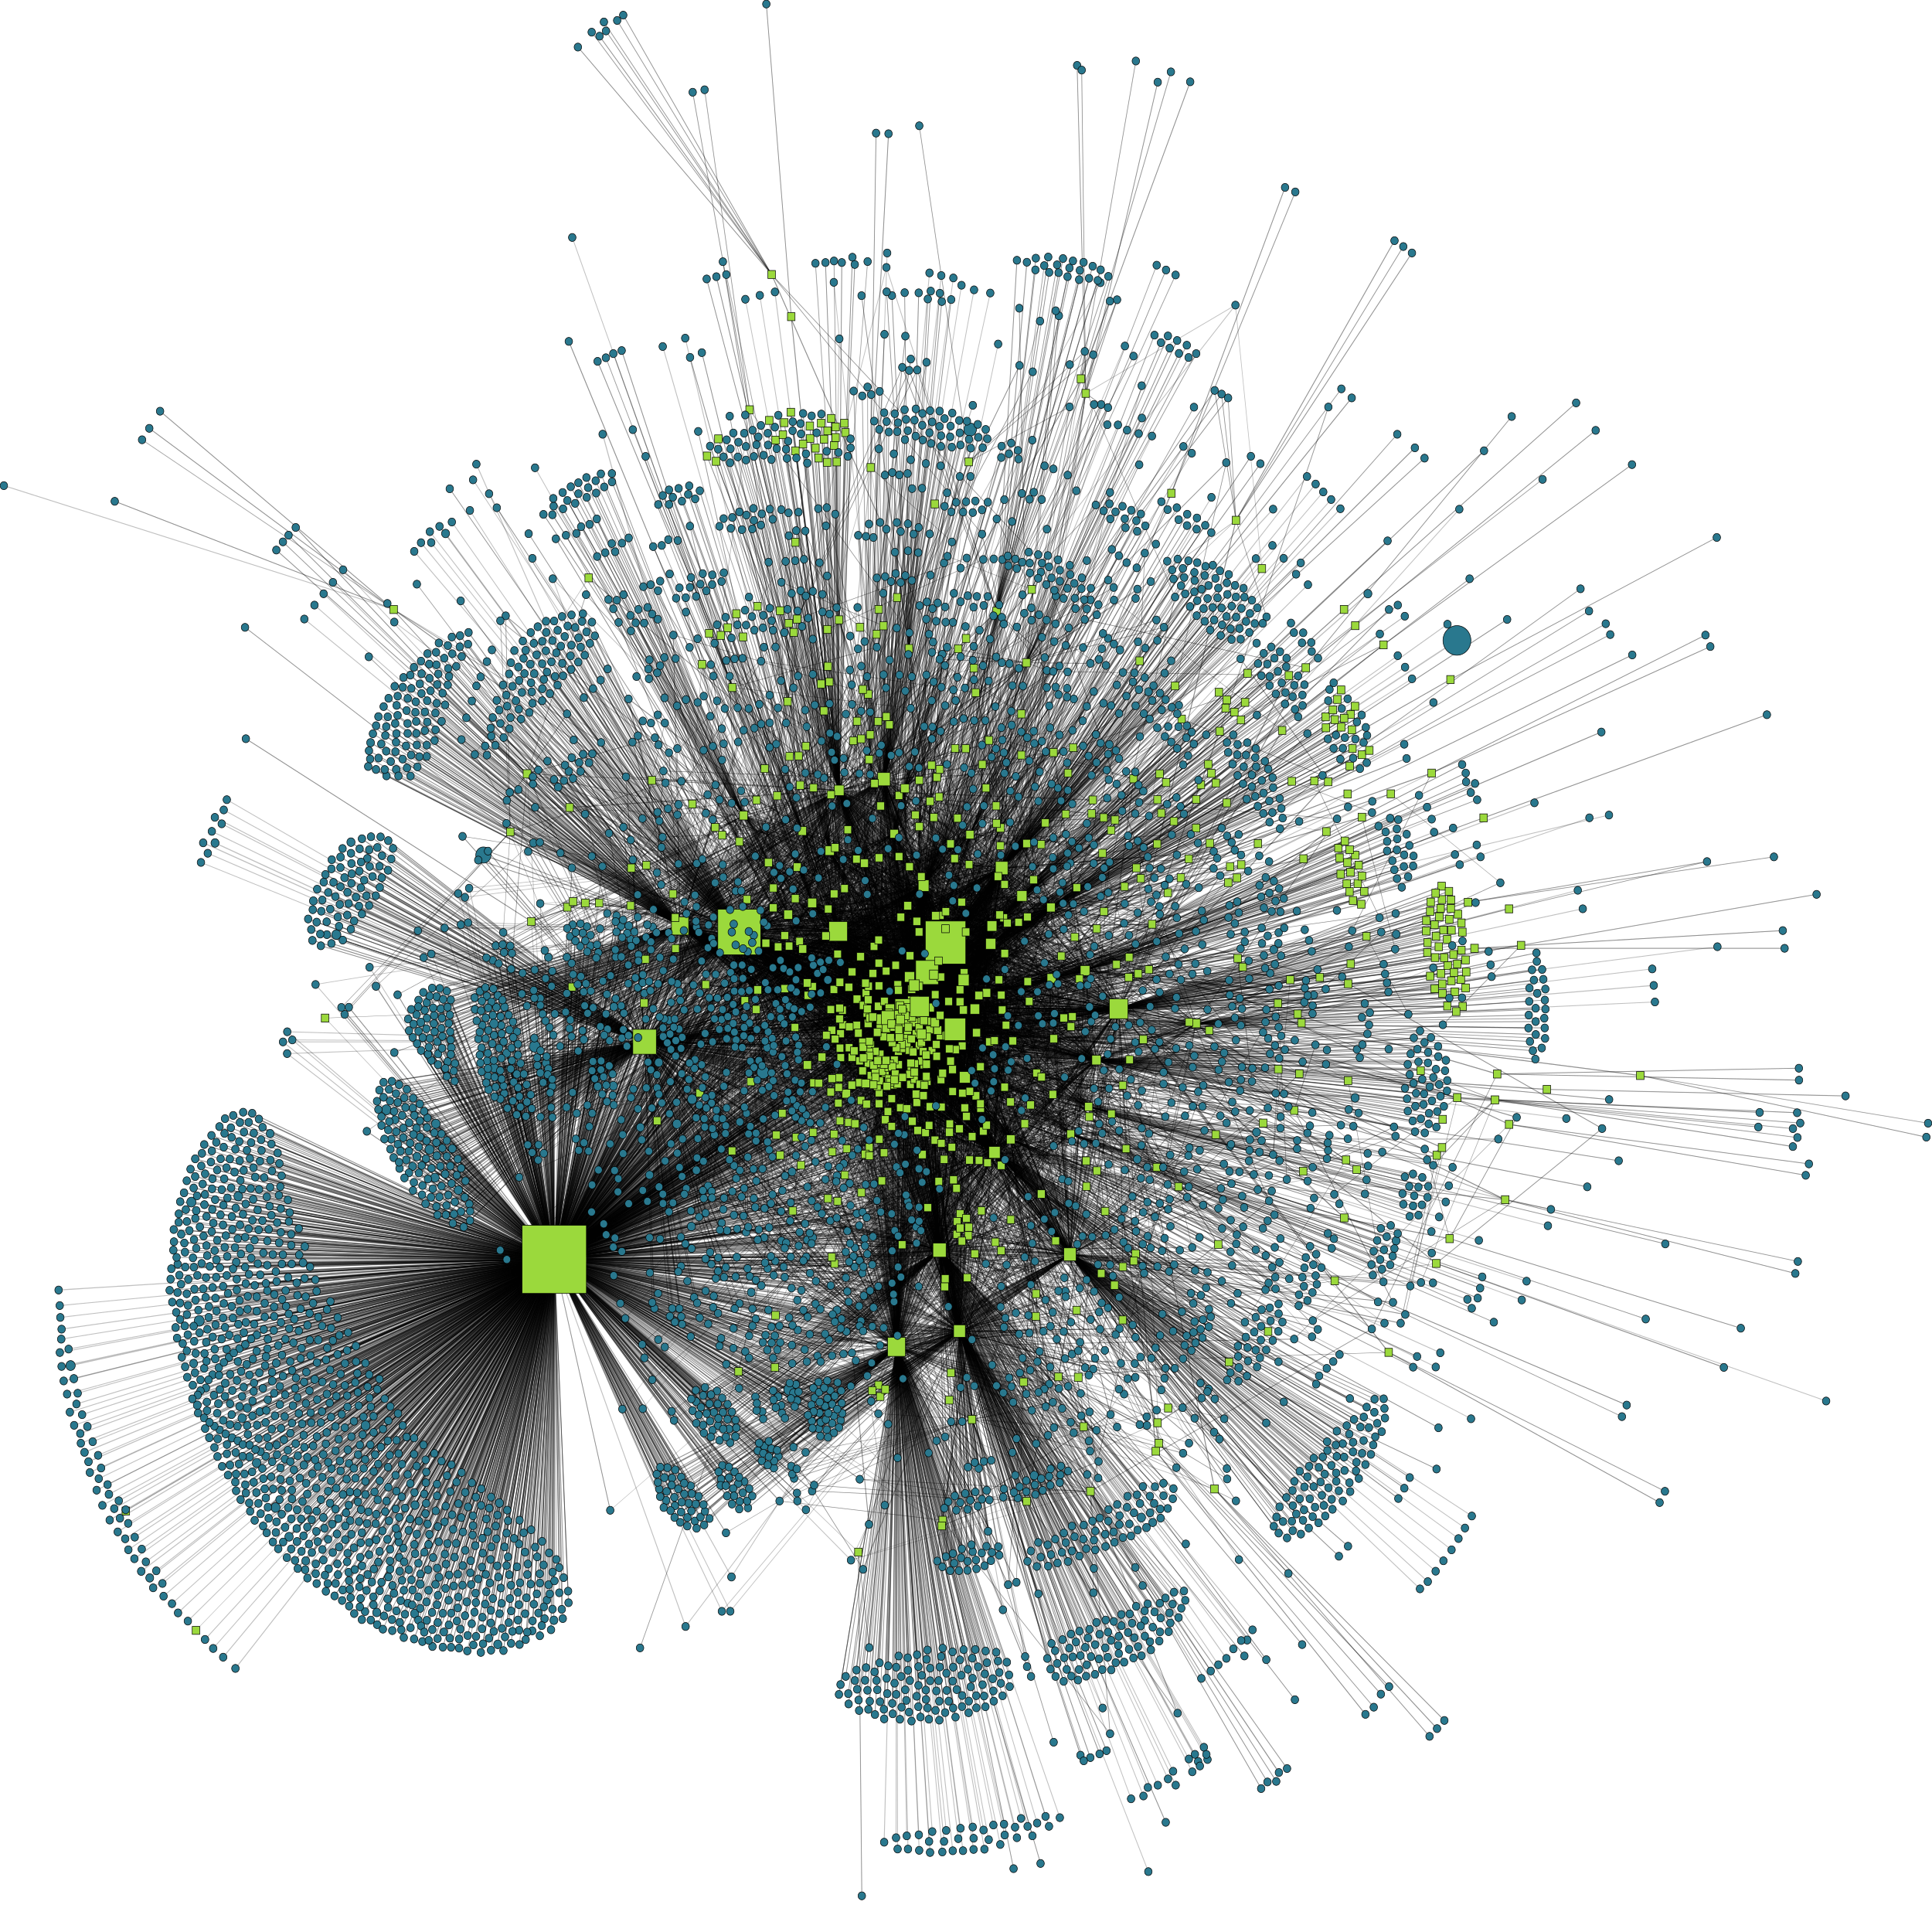
\includegraphics[width=0.8\textwidth]{./img/5kFull.png}
% 	\end{center}
% \end{frame}


\subsection{Ergebnisse}
% Network plot - Colorscale DebtRank
\begin{frame}[fragile,plain]
	\begin{tikzpicture}
		\draw[draw=white] (-0.2,-1.2) rectangle(8.8,0.5);
		\begin{axis}[hide axis,scale only axis,height=0pt,width=0pt,colormap/viridis,colorbar, point meta min=0,point meta max=0.7,colorbar style={height=0.7\textwidth,ytick={0,0.1,...,0.7,0.7}}]
		\addplot [draw=none] coordinates {(0,0)};
		\end{axis}
		\node[anchor=north east] (img) at(0,-0.45) {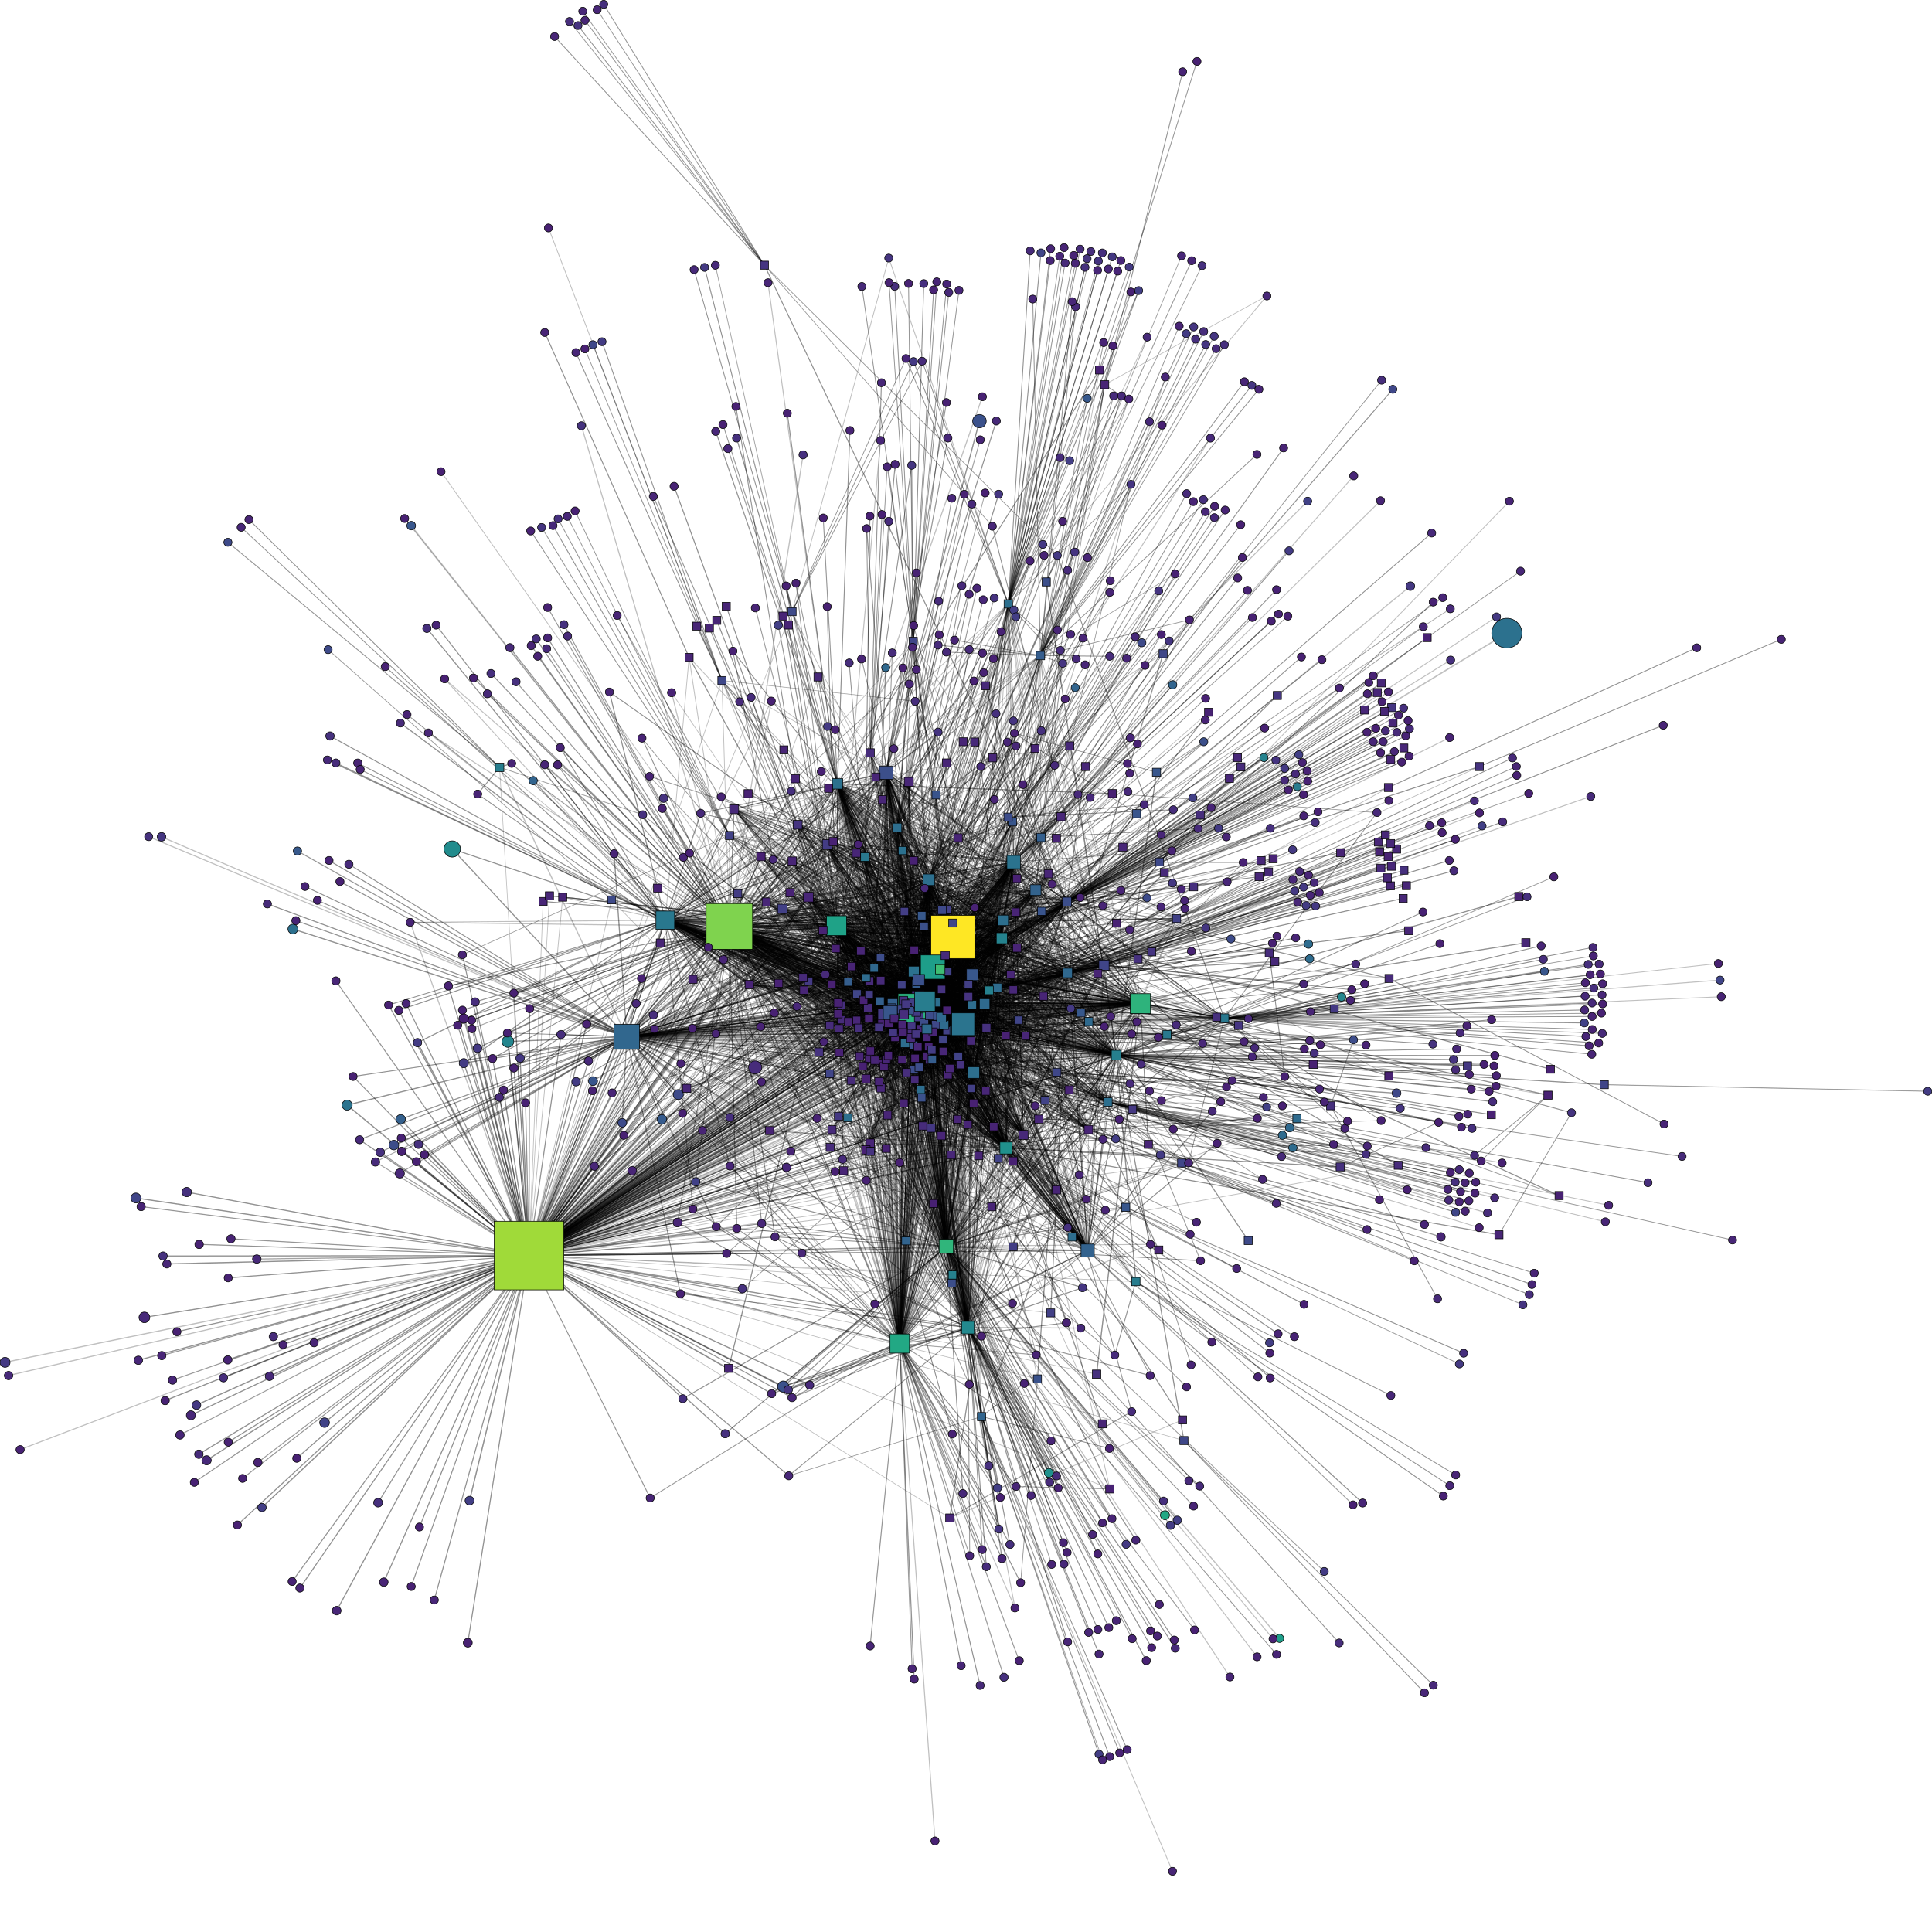
\includegraphics[width=0.8\textwidth]{./img/5kDR.png}};
		\node[anchor=north ] (label) at(0,0.75) {DebtRank $R^F$:};
	\end{tikzpicture}
\end{frame}

% DebtRank plot - Companies & Banks ranked
\begin{frame}[plain,fragile]
	\def\CUTOFF{35.05}
	\def\BarWidth{6pt}
	\def\WIDTH{350pt}
	\def\HEIGHT{135pt}
	\hspace*{-\beamerleftmargin}\begin{tikzpicture}[]
	\node[anchor=south west] (A) at (0,0){
	\begin{tikzpicture}[]
	\def\file{./data/5000c/drSortedBoth.csv}
	\pgfplotstableread[col sep=tab,trim cells]{\file}\table
	\begin{axis}[clip marker paths=true,% axis on top=true
	, 	height=\HEIGHT
	,	width=\WIDTH
	,	ylabel near ticks
	,	ylabel={DebtRank}
	,	xlabel={Companies \& banks ranked by DebtRank}
	,	ylabel style={xshift=-7pt, yshift=-3pt}
	,	xlabel style={yshift=10pt}
	,	scaled y ticks = false
	,	ymin = 0,	ymax =0.75
	,	ytick = {0,0.25,0.50,0.7}
	,	yticklabels = {0.0,0.25,0.50,0.70}
	,	xmin = 0, xmax = \CUTOFF % 35 bis Flughafen Wien
	,	bar width= \BarWidth
	,	ybar =-\BarWidth
	,	major grid style={thin,dashed,black!20}
	,	every node near coord/.append style={anchor=west, rotate=50,font=\scriptsize, fill = black, inner sep = 0.5pt, xshift = 3pt, rounded corners}
	,	x tick style={opacity=0}
	,	y tick style={opacity=0}
	,	cycle list name=onaceColors
	%,	axis y line*=left
	%,	axis x line*=bottom
	,	xtick = \empty
	,	ymajorgrids,
	,	major grid style={thin,dashed,black!20}
	,	legend pos=north east
	,	legend style={fill=white, fill opacity=0.9, draw opacity=1,text opacity=1}
	,	legend cell align=left
	,	every node near coord/.append style={anchor=west,font=\scriptsize}
	,	cycle list name=compBankList
	]
	\addplot+[
		, point meta=explicit symbolic,
		, discard if not={bank}{0},
		, yticklabels from table={\table}{label}
		] table[
		, trim cells
		, x expr= \coordindex + 0.5
		, y =debtrank
		, meta=label
		] from \file;
	\addlegendentry{Companies}
	\addplot+[
		,   point meta=explicit symbolic
		,   discard if not={bank}{1}
		,   yticklabels from table={\table}{label}
		] table[
		,   trim cells
		,   x expr= \coordindex  + 0.5
		,   y =debtrank
		] from \file;
	\addlegendentry{Banks}
	\end{axis}
	\end{tikzpicture}};
	\uncover<2->{\node[anchor=north west,xshift=0pt](B) at (0,0) {\begin{tikzpicture}[]
	\def\file{./data/5000c/drSortedComp.csv}
	\pgfplotstableread[col sep=tab,trim cells]{\file}\table
	\begin{axis}[clip marker paths=true,% axis on top=true
	, 	height=\HEIGHT
	,	width=\WIDTH
	,	ybar
	,	ylabel={DebtRank}
	,	xlabel={Companies ranked by DebtRank}
	,	ylabel style={xshift=-34pt, yshift=5pt}
	,	xlabel style={yshift=5pt}
	,	ymin = 0,	ymax =0.75
	,	ytick = {0,0.25,0.50,0.7}
	,	yticklabels = {0.0,0.25,0.50,0.70}
	,	xmin = 0, xmax = \CUTOFF % 35 bis Flughafen Wien
	,	ymajorgrids,
	,	bar width= \BarWidth
	,	ybar =-\BarWidth
	,	major grid style={thin,dashed,black!20}
	,	legend columns=5, 
	,	legend style={fill=white, fill opacity=0.95, draw opacity=1,text opacity=1, font=\scriptsize}
	,	legend cell align=left
	,	every node near coord/.append style={anchor=west, rotate=50,font=\tiny, fill = black, inner sep = 0.5pt, xshift = 2pt, yshift=3pt, rounded corners=2pt}
	,	x tick style={opacity=0}
	,	y tick style={opacity=0}
	,	cycle list name=onaceColors
	,	xtick = data % add ONACE as xTICK
	,	xticklabels from table={\table}{o} % o = 1 ona = 3 digits of ONACE
	,	xticklabel style={font=\footnotesize\ttfamily\bfseries, anchor=north,yshift=5pt}
	, ]
	\addplot[forget plot
		,	draw=none
		,	point meta=explicit symbolic,
		,	xtick = data
		,	xticklabels from table={\table}{o}
		]table[
		,	trim cells
		,	x expr= \coordindex +0.5
		,	y =debtrank
		,	meta=o
		] from \file;
	\foreach \i in {0,...,9}{
		\addplot+[
		,	nodes near coords
		,	nodes near coords align={vertical},
		,	point meta=explicit symbolic,
		,	discard if not={idx}{\i}
		]table[
		,	trim cells
		,	x expr= \coordindex +0.5
		,	y =debtrank
		,	meta=label
		] from \file;
	}
	\addlegendentry{M Services}
	\addlegendentry{K Finance}
	\addlegendentry{F Construction}
	\addlegendentry{L Immo}
	\addlegendentry{N Other}
	\addlegendentry{H Logistics}
	\addlegendentry{G Automobile}
	\addlegendentry{D Energy}
	\addlegendentry{I Gastronomy}
	\addlegendentry{Q Health}
	\end{axis}
	\end{tikzpicture}};}
	\end{tikzpicture}
\end{frame}

% Scatter 
% \begin{frame}[fragile,plain]
% 	\newcommand{\defZoom}[4]{\def\XMIN{#1}\def\XMAX{#2}\def\YMIN{#3}\def\YMAX{#4}}
% 	\defZoom{1E8}{1E10}{0.16}{0.6}
% 	\vspace*{-8pt}
% 	\hspace*{-\beamerleftmargin}% !TeX root = ../../MScBeamer.tex
\def\File{./data/\NWSize/LiabilitiesDebtRank.txt}
\begin{tikzpicture}
\begin{axis}[
,	scale  only  axis
,	axis y line*=left% the ’*’ avoids arrow heads
,	height=90pt
,	xmode=log
,	width=0.35\paperwidth
,	xlabel={Liabilities (EUR)} 
,	ylabel={DebtRank}
,	ylabel style={yshift=-10pt}
,	ticks=major
%,	xmajorgrids
%,	enlargelimits=false
, 	major grid style={line width=0.1pt,draw=gray!30}
,	xmin = 1E5
,	xmax = 1E11
%,	ymin= 0
%,	ymax=0.75
,	legend cell align=left
,	legend pos=north west
,	legend image post style={scale=2.5}
]
\addplot[bankColor
	,	only marks
	,	discard if not={Bank}{1}
	,	mark size=1pt
	]table[
		x = Liabilities
	,	y = DebtRank
	,	filter discard warning=false
	]{\File};\addlegendentry{Banks}%\label{plt:scattercost}
\addplot[companyColor
	,	only marks
	,	discard if not={Bank}{0}
	,	mark size=1pt
	]table[
		x = Liabilities
	,	y = DebtRank
	,	filter discard warning=false
	]{\File};\addlegendentry{Companies}%\label{plt:scattercost}
\draw [dashed, thick,rounded corners=3pt] (axis cs:\XMIN,\YMIN) rectangle (axis cs:\XMAX,\YMAX);
\end{axis}
\end{tikzpicture}%
% 	% !TeX root = ../../MScBeamer.tex
\def\File{./data/\NWSize/LiabilitiesDebtRank.txt}
\begin{tikzpicture}
\begin{axis}[
,	scale  only  axis
,	axis y line*=left % the ’*’ avoids arrow heads
,	height=90pt
,	xmode=log
,	width=0.35\paperwidth
,	xlabel={Liabilities (EUR)} 
,	ylabel={}
,	ticks=major
, 	major grid style={line width=0.1pt,draw=gray!30}
,	xmin = \XMIN
,	xmax = \XMAX
,	ymin = \YMIN
,	ymax = \YMAX
,	legend cell align=left
,	legend pos=north west
,	legend image post style={scale=1.25}
]
\addplot[bankColor
	,	only marks
	,	discard if not={Bank}{1}
	,	mark size=1.5pt
	]table[
		x = Liabilities
	,	y = DebtRank
	,	filter discard warning=false
	]{\File};
\addplot[companyColor
	,	only marks
	,	discard if not={Bank}{0}
	,	mark size=1.5pt
	]table[
		x = Liabilities
	,	y = DebtRank
	,	filter discard warning=false
	]{\File};
\end{axis}
\end{tikzpicture}

% 	\defZoom{2E7}{5E10}{0.05}{0.4}
% 	\vspace*{-16pt}\hspace*{-\beamerleftmargin}% !TeX root = ../../MScBeamer.tex
%\pgfplotstableread{./data/BilanzsummeDebtrank.txt}\loadedtable
\def\File{./data/\NWSize/BilanzsummeDebtrankBankCompanies.txt}
\begin{tikzpicture}
\begin{axis}[
,	scale  only  axis
,	axis y line*=left% the ’*’ avoids arrow heads
,	height=90pt
,	xmode=log
,	width=0.35\paperwidth
,	xlabel={Total assets (EUR)} 
,	ylabel={DebtRank}
,	ylabel style={yshift=-10pt}
,	ticks=major
%,	xmajorgrids
%,	enlargelimits=false
, 	major grid style={line width=0.1pt,draw=gray!30}
,	xmin = 1E4
,	xmax = 1E12
%,	ymin= 0
%,	ymax=0.75
,	legend cell align=left
,	legend pos=north west
,	legend image post style={scale=2.5}
]
\addplot[bankColor
	,	only marks
	,	discard if not={Bank}{1}
	,	mark size=1pt
	]table[
		x = TotalAssets
	,	y = DebtRank
	,	filter discard warning=false
	]{\File};\addlegendentry{Banks}%\label{plt:scattercost}
\draw [dashed, thick,rounded corners=3pt] (axis cs:\XMIN,\YMIN) rectangle (axis cs:\XMAX,\YMAX);
\addplot[companyColor
	,	only marks
	,	discard if not={Bank}{0}
	,	mark size=1pt
	]table[
		x = TotalAssets
	,	y = DebtRank
	,	filter discard warning=false
	]{\File};\addlegendentry{Companies}%\label{plt:scattercost}
\end{axis}
\end{tikzpicture}%
% 	% !TeX root = ../../MScBeamer.tex
%\pgfplotstableread{./data/BilanzsummeDebtrank.txt}\loadedtable
\def\File{./data/\NWSize/BilanzsummeDebtrankBankCompanies.txt}
\begin{tikzpicture}
\begin{axis}[
,	scale  only  axis
,	axis y line*=left% the ’*’ avoids arrow heads
,	height=90pt
,	xmode=log
,	width=0.35\paperwidth
,	xlabel={Total assets (EUR)} 
,	ylabel={}
,	ticks=major
%,	xmajorgrids
%,	enlargelimits=false
, 	major grid style={line width=0.1pt,draw=gray!30}
,	xmin = \XMIN
%,	xmax = \XMAX
,	ymin= \YMIN
%,	ymax=\YMAX
,	legend cell align=left
,	legend pos=north west
%,	cycle list name=compBankList,
,	legend image post style={scale=1.25}
]

\addplot[bankColor
	,	only marks
	,	discard if not={Bank}{1}
	,	mark size=1.5pt
	]table[
		x = TotalAssets
	,	y = DebtRank
	,	filter discard warning=false
	]{\File};%\addlegendentry{Banks}%\label{plt:scattercost}
\addplot[companyColor
	,	only marks
	,	discard if not={Bank}{0}
	,	mark size=1.5pt
	]table[
		x = TotalAssets
	,	y = DebtRank
	,	filter discard warning=false
	]{\File};%\addlegendentry{Companies}%\label{plt:scattercost}
\end{axis}
\end{tikzpicture}

% \end{frame}


\begin{frame}{Zusammenfassung}
	\begin{itemize}
		\item Verwendete Methoden inspiriert von stochastischen Prozessen um das systemische Risiko von Firmen und Banken eines Landes zu quantifizieren
		\bigskip
		\item Systemisches Risiko von Interbank Netzwerk unterschätzt das reale Risiko (nur 29\% des absoluten Betrages)
		\item Im vollständigen Netzwerk beträgt der Beitrag der Firmen zum systemischen Risko 55\%
%		\item Extending policies against systemic risk for companies may be worthwhile
	\end{itemize}
\end{frame}



\appendix

		%\subsection{References}
\begin{frame}[allowframebreaks]{References}
	\nocite{newman_networks:_2010}
	\bibliography{references}
%	\bibliography{defensio}
\end{frame}


\begin{frame}{Centrality Measures}
	Details from centrality measures mentioned previously
	\begin{itemize}
		\item Katz centrality: Not only sum of centralities of nearest neighbors but also the centrality of nodes at arbitrary distance $k$ taken into account (with a factor $\alpha^k$ where $\alpha<1$):
		\begin{align*}
		C_K(v_i) &= \sum_{\alert<3>{k=1}}^\infty\sum_{v_j\in V}\alpha^k (A^k)_{ij} \qquad
		&&
%			\frac{1}{1-\alpha x} &= 1 + \alpha x + (\alpha x)^2 + (\alpha x)^3 + \ldots = \sum_{\alert<2>{k=0}}^\infty (\alpha x)^k\quad\\
			\vec K = ((I - \alpha A)^{-1} \alert<3>{-I})\cdot\vec I
		\end{align*}
		\item PageRank: Divide centrality contribution of node by the number of outgoing links (with $D_{ij} = \delta_{ij}\mathrm{max}(1,k_j^\text{out})$)
		\begin{align*}
			C_P(v_i) &=  \alpha\sum_{k=1}^N A_{ij}\frac{x_j}{k_j^\text{out}} +  \beta\qquad
			&&
			\vec P = D(D - \alpha A)^{-1}\cdot\vec I
		\end{align*}
	\end{itemize}
\end{frame}	

\begin{frame}{DebtRank}
	\begin{itemize}[<+-| alert@+>]
		\item Nodes have three states, undistressed (U), distressed (D) and inactive (I) and a distress level $\in [0,1]$. Initially, all nodes start in state U.
		\item Nodes are connected with weighted arcs, $W_{ij} = \mathrm{min}\left(\frac{L_{ij}}{C_j},1\right)$
		\item To measure the impact of default from a set of nodes the distress level of those nodes is set to $1$.
		\item Nodes go into state D (distressed) if a neighboring node ($W_{ij} > 0$) is in distress
		\item If a node has been in distress in the previous timestep it will be inactive from then on ($\Rightarrow$ no loops)
	\end{itemize}	
\end{frame}
\begin{frame}{DebtRank: Example ($W_{ij} = 0.5$)}
	% !TeX root = ../MSc.tex
\def\sfScale{1.7}
\def\hDist{5}
\def\vDist{6.9}
\newcommand{\drNode}[5][]{\node[minimum size=1cm, circle split part fill={#4,#4,drMap},#1] (#2) at #3 {#2 #5\nodepart{lower}#4};}
\begin{tikzpicture}[
    , very thick
    , font={\fontsize{11pt}{11pt}\bfseries}
    , circle split draw splits=false
    , inner sep=2pt
    , shape=circle split
    , Edge/.style={thick,-{Latex[length=3mm, width=1.5mm]}}] 
% \draw(-7.0,-\vDist) rectangle(7.11,\vDist+0.1);
\clip(-7.0,-\vDist) rectangle(7.11,\vDist+0.1);
\node(a) at (-\hDist,0){
    \begin{tikzpicture}[scale=\sfScale]
    \drNode{1}{(2,5)}{1.0}{D}
    \foreach \a in {2,...,4}{
      \drNode{\a}{(\a*0.8-0.4,4)}{0.0}{U}
      \path[Edge](1) edge (\a);
    } 
    \drNode{5}{(1+0.2,2.85)}{0.0}{U}
    \drNode{6}{(3-0.2,2.85)}{0.0}{U}
    \path[Edge](5) edge[bend left=25] (2);
    \path[Edge](2) edge[bend left=25] (5);
    \path[Edge](4) edge (6);
    \path[Edge](6) edge (5);

    \drNode{7}{(1.2,1.75)}{0.0}{U}
    \drNode{8}{(2.8,1.75)}{0.0}{U}
    \path[Edge](5) edge (7);
    \path[Edge](6) edge (8);
    \node[left of=1, node distance = 1.4cm,yshift=0.225cm]{Time: 1};
    \end{tikzpicture}
};
\node(b) at (-0.1,0){
    \begin{tikzpicture}[scale=\sfScale]
    \drNode{1}{(2,5)}{1.0}{I}
    \foreach \a in {2,...,4}{
      \drNode{\a}{(\a*0.8-0.4,4)}{0.5}{D}
      \path[Edge](1) edge (\a);
    } 
    \drNode{5}{(1.2,2.85)}{0.0}{U}
    \drNode{6}{(2.8,2.85)}{0.0}{U}
    \path[Edge](5) edge[bend left=25] (2);
    \path[Edge](2) edge[bend left=25] (5);
    \path[Edge](4) edge (6);
    \path[Edge](6) edge (5);

    \drNode{7}{(1.2,1.75)}{0.0}{U}
    \drNode{8}{(2.8,1.75)}{0.0}{U}
    \path[Edge](5) edge (7);
    \path[Edge](6) edge (8);
    \node[left of=1, node distance = 1.7cm,yshift=0.225cm]{Time: 2};
    \end{tikzpicture}
};
\node(c) at (\hDist-0.2,0){
    \begin{tikzpicture}[scale=\sfScale]
    \drNode{1}{(2,5)}{1.0}{I}
    \foreach \a in {2,...,4}{
      \drNode{\a}{(\a*0.8-0.4,4)}{0.5}{I}
      \path[Edge](1) edge (\a);
    } 
    \drNode[inner sep = 1pt]{5}{(1.2,2.85)}{0.25}{D}
    \drNode[inner sep = 1pt]{6}{(2.8,2.85)}{0.25}{D}
    \path[Edge](5) edge[bend left=25] (2);
    \path[Edge](2) edge[bend left=25] (5);
    \path[Edge](4) edge (6);
    \path[Edge](6) edge (5);

    \drNode{7}{(1+0.2,1.75)}{0.0}{U}
    \drNode{8}{(3-0.2,1.75)}{0.0}{U}
    \path[Edge](5) edge (7);
    \path[Edge](6) edge (8);
    \node[left of=1, node distance = 1.7cm,yshift=0.225cm]{Time: 3};
    \end{tikzpicture}
};
\node[xshift=-1.3cm](d) at (0.1,-\vDist){ %-\hDist/2
    \begin{tikzpicture}[scale=\sfScale]
    \drNode{1}{(2,5)}{1.0}{I}
    \foreach \a in {3,...,4}{
      \drNode{\a}{(\a*0.8-0.4,4)}{0.5}{I}
      \path[Edge](1) edge (\a);
    }
    \drNode[inner sep=.5pt]{2}{(0.8*2-0.4,4)}{0.625}{I}
    \path[Edge](1) edge (2);
    \drNode[inner sep=.5pt]{5}{(1.2,2.85)}{0.375}{I}
    \drNode[inner sep=1pt]{6}{(2.8,2.85)}{0.25}{I}
    \path[Edge](5) edge[bend left=25] (2);
    \path[Edge](2) edge[bend left=25] (5);
    \path[Edge](4) edge (6);
    \path[Edge](6) edge (5);

    \drNode[inner sep=.5pt]{7}{(1.2,1.75)}{0.125}{D}
    \drNode[inner sep=.5pt]{8}{(2.8,1.75)}{0.125}{D}
    \path[Edge](5) edge (7);
    \path[Edge](6) edge (8);

    \node[left of=1, node distance = 1.7cm,yshift=0.225cm]{Time: 4};
    \node[left of=2, node distance = 2cm,yshift=-0.25cm]{$\boldmath h_2 = \nicefrac12+\nicefrac14$};
    \node[left of=5, node distance = 2cm,yshift=-0.25cm]{$\boldmath h_5 = \nicefrac14+\nicefrac18$};
    \end{tikzpicture}
};
\node(e) at (\hDist-0.2,-\vDist){ % \hDist/2
    \begin{tikzpicture}[scale=\sfScale]
    \drNode{1}{(2,5)}{1.0}{I}
    \foreach \a in {3,...,4}{
      \drNode{\a}{(\a*0.8-0.4,4)}{0.5}{I}
      \path[Edge](1) edge (\a);
    }
    \drNode[inner sep=.5pt]{2}{(0.8*2-0.4,4)}{0.625}{I}
    \path[Edge](1) edge (2);
    \drNode[inner sep=.5pt]{5}{(1.2,2.85)}{0.375}{I}
    \drNode[inner sep=1pt]{6}{(2.8,2.85)}{0.25}{I}
    \path[Edge](5) edge[bend left=25] (2);
    \path[Edge](2) edge[bend left=25] (5);
    \path[Edge](4) edge (6);
    \path[Edge](6) edge (5);

    \drNode[inner sep=.5pt]{7}{(1.2,1.75)}{0.125}{I}
    \drNode[inner sep=.5pt]{8}{(2.8,1.75)}{0.125}{I}
    \path[Edge](5) edge (7);
    \path[Edge](6) edge (8);
    \node[left of=1, node distance = 1.7cm,yshift=0.225cm]{Time: 5};
    \end{tikzpicture}
};
\drNode{3}{(-6.1,1-\vDist)}{0.2}{D}
\node[above of=3](I){Index $i$};
\node[right of=3,node distance = 2.25cm,yshift=0.25cm](S){Status $s_i(t)$};
\node[right of=3,node distance = 2.25cm,yshift=-0.7cm](D){Distress $h_i(t)$};

\coordinate(I) at (I);
\coordinate(S) at (S.west);
% \coordinate(D) at (D.west);
\draw(-6.3,1.4-\vDist) --(I);
\draw(-5.7,1.25-\vDist) --($(S) + (0,0.2)$);
\draw(-5.7,0.75-\vDist) --(D);

\draw (I)++(0.5:260);
\end{tikzpicture}	
\end{frame}

\begin{frame}%{Empirical data}
	% !TeX root = ../MSc.tex
\begin{tikzpicture}[]
\def\file{./data/histLiabTransposed.csv}
 \pgfplotstableread[col sep=tab,trim cells]{\file}\table
%\pgfplotstableread[col sep=tab,trim cells]{\fileB}\tableB
%\pgfplotstableread{./data/returnhistF.csv}\loadedtableF
\begin{axis}[width=\iftoggle{thesis}{1.0}{0.53}\textwidth
,	height=350pt
,	xbar stacked
,	xlabel={Sum of liabilities (EUR)}
,	ylabel={Liability types ordered by their total sum}
,	ylabel style={yshift=-25pt}
%,	border={1pt 1pt 1pt 0pt}
%,	ytick=data
,	ytick = \empty
%,	xtick = {1E11,...,5E11}
%,	yticklabels from table={\table}{name}
,	every node near coord/.append style={rotate=0, anchor=west,font=\footnotesize  }
%,	scaled x ticks = false
,	xmajorgrids,
%,	axis x line*=bottom
,	axis y line*=left
%,	hide y axis
,	bar width= 8pt
,	xmin = 0
,	xmax = 5.5E11
,	ymax = 0
,	ymin =-31
,	x tick style={opacity=0}
,	major grid style={thin,dashed,black!20}
,	legend pos=south east
,	legend style={fill=white, fill opacity=0.9, draw opacity=1,text opacity=1, draw = none}
,	legend style={
		,	fill=white
		,	draw opacity=1
		,	text opacity=1
		% ,	draw=none
		% ,	legend columns=-1
		% % ,	fill opacity=0.9
		% ,	column sep=0.28ex
		% ,	yshift=8pt
		% ,	xshift=8pt
	}
% ,	legend image post style={xscale=1.65,yscale=1.8}
,	legend image post style={xscale=1.4,yscale=1.4}
,	legend cell align=left
,	cycle list name=connCountList
,	]
\pgfplotsinvokeforeach{0,1,...,5}
{
\addplot+[]
	table[trim cells,y expr= -\coordindex+0.5, x =c#1] from \file;\label{plt:liab#1}\addlegendentry{{#1 Bank\ifthenelse{#1 = 1}{}{s}}}
}
\addplot+[nodes near coords,nodes near coords align={vertical},
	point meta=explicit symbolic] 
	table[trim cells,y expr= -\coordindex+0.5, x =c6, meta = name] from \file;
	\addlegendentry{{6 Banks}} 
\end{axis}
% white rectangles to hide dotted lines
% \draw[fill=white,draw=none](6.5,1.1) rectangle(16,5);
% \draw[fill=white,draw=none](8,0.65) rectangle(13,0.2);
% \node[] at (11,2.5) {% !TeX root = ../MSc.tex
\begin{tikzpicture}[]

\def\file{./data/bankCountHist.csv}
 \pgfplotstableread[col sep=tab,trim cells]{\file}\table
% \pgfplotstableread{./data/returnhistF.csv}\loadedtableF
  \begin{axis}[width=0.5\textwidth
,	height=130pt
,	ybar
,	xlabel={Number of bank connections}
,	ylabel={Company count}
,	every node near coord/.append style={rotate=0, anchor=south,font=\footnotesize}
%,	xticklabels from table={\loadedtable}{label},
%,	flexible xticklabels from table={\file}{label}{col sep=tab}
,	xticklabel style={text height=1.5ex} % To make sure the text labels are nicely aligned
,	xtick={0,1,2,3,4,5,6}
,	ytick={0,25000,50000}
,	scaled x ticks = false
,	ymin = 0,	ymax =55000
%,	xmin = 0, xmax = 29
,	ymajorgrids
,	axis y line*=left
,	bar width= 15pt
,	ybar =-15pt
%,	hide x axis
,	axis x line*=bottom,
,	axis y line*=right
, ylabel near ticks
, yticklabel pos=right
,	major grid style={thin,dashed,black!20}
,	scaled y ticks = false
%,	ylabel style={yshift=\iftoggle{thesis}{15pt}{5pt}}
,	xtick style={opacity=0}
,	ytick style={opacity=0}
,	y tick label style=
		{/pgf/number format/fixed
		,/pgf/number format/1000 sep = \thinspace % replace comma as 1000 separator 
		}
,	cycle list name=connCountList,
%,	legend pos=south west
%,	legend style={fill=white, fill opacity=0.9, draw opacity=1,text opacity=1}
%,	legend cell align=left
 ]
  \pgfplotsinvokeforeach{0,1,2,3,4,5,6}{
	\addplot+[nodes near coords,nodes near coords align={vertical},
		point meta=explicit symbolic]	table[trim cells,x expr=#1, y index =#1, meta index= #1] from \file;
    }
%	\addlegendentry{\#Companies }
  \end{axis}
\end{tikzpicture}};% small plot in plot

\end{tikzpicture}
\end{frame}





% \pgfmathdeclarefunction{diffglg}{3}{\pgfmathparse{1/(sqrt(4*pi*#2*#3))*exp(-((x-#1)^2)/(4*#2*#3))}}
% \begin{frame}{Diffusion in 1 dimension }
% 	\begin{tikzpicture}
% 		\begin{axis}[
% 			,	no markers
% 			,	domain=-0:5
% 			,	samples=\SAMPLESONE
% 			,	thick
% 			,	axis lines*=left
% 			,	xlabel=$x$
% 			,	ylabel={$f(x,t)$}
% 			,	every axis y label/.style={at=(current axis.above origin),anchor=south},
% 			%,	every axis x label/.style={at=(current axis.right of origin),anchor=west},
% 			,	xlabel style={yshift=15pt}
% 			,	height=5cm, width=10cm
% 			,	xtick={0}
% 			,	ytick=\empty
% 			,	enlargelimits=false
% 			,	clip=false
% 			,	axis on top
% 			%	,	grid = major
% 			,	]
% 			%		  \addplot [fill=cyan!20, draw=none, domain=0:5.96] {diffglg(1,3)} \closedcycle;
% 			% \pgfplotsinvokeforeach{0,1,...,5}{
% 			% 	\addplot [very thick,cyan!50!black] {diffglg(0,0.01,#1)};
% 			% }
			
% 			\foreach \i in {80,160,...,900} {
% 			\edef\temp{\noexpand\addplot [very thick,color of colormap={\i}] {diffglg(0,0.001,\i)};}
% 			\temp
% 			}
% 			\draw[ultra thick,color of colormap=0] (axis cs:0,0) -- (axis cs:0,1.05);
% 			\addplot [very thick,red!50!black] {diffglg(0,0.1,1000)};
% 			%	\addplot [very thick,cyan!50!black] {diffglg(0,0.001)};
% 			%\addplot [very thick,cyan!50!black] {diffglg(0,0.001)};
% 			%\addplot [very thick,cyan!50!black] {diffglg(0,1)};
% 		\end{axis}
		
% 	\end{tikzpicture}
% \end{frame}
\end{document} 
